\documentclass[a4paper, 11pt]{article}

\usepackage[version=3]{mhchem}
\usepackage{siunitx}
\usepackage{graphicx}
\usepackage{amsmath}
\usepackage[total={16cm,25cm}, top=3cm, left=2.5cm, includefoot]{geometry}
\usepackage{pgfplots}
\usepackage{float}
\usepackage{amsfonts}
\usepackage{booktabs}
\usepackage{easytable}
\usepackage{mathtools}
\usepackage{comment}
\usepackage[makeroom]{cancel}
\renewcommand{\figurename}{Obrázek}
\renewcommand{\refname}{Zdroje}
\renewcommand{\tablename}{Tabulka}
\renewcommand{\contentsname}{Obsah}

\setlength\parindent{0pt}
\setcounter{section}{0}
\renewcommand{\labelenumi}{\alph{enumi}.}
\usepackage{xcolor}
\definecolor{light-gray}{gray}{0.95}
\newcommand{\code}[1]{\colorbox{light-gray}{\texttt{#1}}}
\newcommand{\logoCVUT}{
\includegraphics[width = 0.5\textwidth]{img/symbol_cvut_konturova_verze_cb.pdf}}
\newcommand{\logoFJFI}{
\includegraphics[width = 0.4\textwidth]{img/fjfi_logo.png}}

\begin{document}
% \include{veličiny}
% \include{zkratky}

% titulní strana
\thispagestyle{empty}

\begin{center}
	{\LARGE
		České vysoké učení technické v Praze \par
		Fakulta jaderná a fyzikálně inženýrská
	}
    \vspace{10mm}

    \begin{tabular}{c}
		\textbf{Katedra jaderných reaktorů} \\[3pt]
    \end{tabular}

   \vspace{10mm} \logoCVUT \vspace{15mm}

   {\huge \textbf{Jaderné inženýrství v praxi}\par}
   \vspace{5mm}
   {\huge \textbf{Magisterské studium}\par}

   \vspace{15mm}
   {\Large \MakeUppercase{Státnicové otázky}}

   \vfill
   {\large
    \begin{tabular}{ll}
    Rok: & 2025
    \end{tabular}
   }
\end{center}

% Prohlášení
\newpage
\thispagestyle{empty}

%~
\vfill

\vspace{1em}

Ahojky, dostávají se ti do rukou státnicové otázky ze předmětu Jaderné inženýrství v praxi. Prosím, měj na paměti, že celkový přehled není v některých tématech ucelený a že se v textu můžou vyskytovat (a stoprocentně vyskytují) chyby jak gramatické, tak faktické. Ale i přestože text má k dokonalosti hodně daleko, předávám ho dál a věřím, že třeba někomu pomůže :)))\\
\\
T.K.\\
\\
No nazdar, jestli tenhle text čteš, tak se ti do rukou dostaly opravené, obohacené, vylepšené a hlavně aktuální otázky dle okruhů na magisterské SZZ v roce 2024. Opět platí to samé co nahoře, je tam spousta chyb, ale snad by měl text poskytovat intenzivnější vhled do problematiky.\\
\\
J.M. + Š.J.\\
\\
Budeme rádi za jakékoli doplnění, opravu nebo komentář a držím palce ke státnicím!!!

\vspace{2em}

\clearpage{\pagestyle{empty}}

\include{none}

\newpage
\parskip=0pt
\begin{small}
\tableofcontents
\end{small}
\parskip=7pt
\newpage

\section[Rentgenofluorescenční analýza]{Energiově a vlnově dispersní rentgenfluorescenční analýza}

\subsection{Princip metody}

Nedestruktivní metoda zjišťování chemického (prvkového) složení zkoumané látky.

Je založena na detekci charakteristického RTG záření, jež je emitováno příslušnými atomy prvků obsažených ve zkoumané látce. Nejprve je látka vystavěna dopadajícím fotonům (RTG záření například z rentgenky nebo gama z vhodného radionuklidu). Tyto fotony pak vyráží elektrony (nejčastěji z vnitřní slupky K, popř. L). Poté dochází k přeskoku elektronů z vyšší slupky na toto prázdné místo a rozdíl energií je vyzářen v podobě fluorescenčních fotonů RTG záření, které je specifické pro daný prvek.

\textbf{Kvalitativní analýza}: je možné díky detekci charakteristického RTG záření, jež je specifické pro daný prvek (detekujeme energii a vlnovou délku).

\textbf{Kvantitativní analýza}: množství emitovaných fotonů charakteristického záření je přímo úměrné množství atomů daného druhu a je tedy mírou koncentrace daného prvku. Kvantita je dána intenzitou jednotlivých píků fluoroscenčního záření.

Vlnová délka charakteristického RTG záření je klesající s rostoucím Z číslem prvků a naopak energie se zvyšuje se $Z$ číslem. Metoda RFA/XRF je dobrá pro prvky s větším $Z$, jelikož se lépe detekují.

\textbf{Výhody:} \begin{itemize}
    \item Rychlost, přesnost a reprodukovatelnost
    \item Vzorky mohou být v jakémkoliv skupenství
    \item Nedestruktivní metoda
    \item Multiprvková analýza
    \item Dobré pro zkoumání složení uměleckých předmětů
\end{itemize}

\textbf{Nevýhody:} \begin{itemize}
    \item Obtížná detekce prvků lehčích než $Z<13$
    \item Nerozpozná chemické sloučeniny
    \item Omezení na pouhý povrch zkoumaného materiálu
\end{itemize}

\begin{figure}[H]
    \centering
    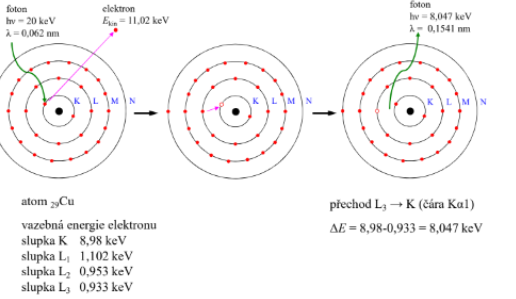
\includegraphics[width=0.9\linewidth]{img/Princip RFA 1.png}
    \caption{Princip RFA 1}
\end{figure}

\begin{figure}[H]
    \centering
    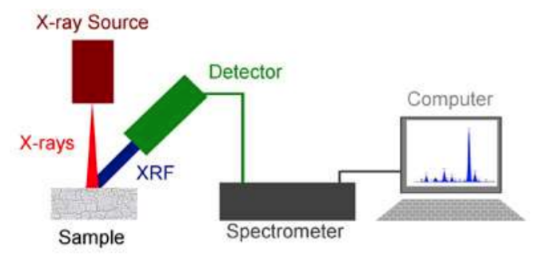
\includegraphics[width=0.7\linewidth]{img/Princip RFA 2.png}
    \caption{Princip RFA 2}
\end{figure}

\subsection{Vlnově disperzní RFA}

Ze skundárního charakteristikcého záření se izolují jednotlivé vlnové délky (čáry) spektra přes difrakci na krystalu. Poté je možné měřit intenzitu jednotlivých čar pro jednotlivé prvky postupně. Pokud máme multikrystal (složen z různých vrstev), pak je možné provádět analýzu současně.

Používá se při kvantitativní analýze prvků B po U (materiál v podobě pevné, zrnité i kapalné)

Vyžaduje velké rozměry přístrojů, vysokou spotřebu energie, ale dosahuje velmi dobrých technických parametrů.

Sekundární záření se odráží na krystalu a dopadá do detektoru/čítače (difrakce je dána Braggovým zákonem).

V závislosti na $Z$ prvků, které chci měřit, tak se volí krystaly:

\begin{itemize}
    \item Pro těžké a středně těžké prvky (= krátké vlnové délky) je používají LiF, NaCl, Ge, InSb.
    \item Pro lehčí prvky se využívají soli organických kyselin s těžkým kovem (ten tvoří uzlové body v krystalové mřížce).
    \item Pro velmi lehké prvky se používají uměle připravené multivrstevnaté krystaly (kde se do matrice lehkého prvku (Si) vkládají vrstvy těžkého kovu).
\end{itemize}

Výsledné spektrum je pak funkcí intenzity na vlnové délce či na difrakčním úhlu $2 \Theta$.

\begin{figure}[H]
    \centering
    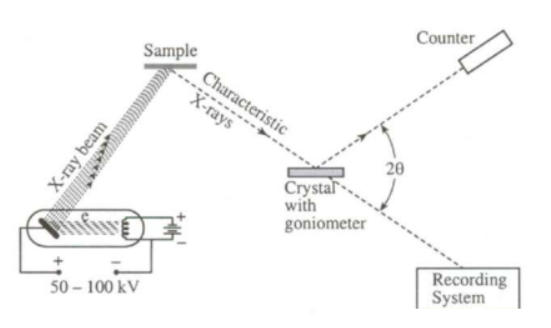
\includegraphics[width=0.8\linewidth]{img/Vlnově_disperzní_RFA.png}
    \caption{Vlnově disperzní RFA}
\end{figure}

\subsection{Energiově disperzní RFA}

Jedná se o menší a levnější přístroje, kde je analyzováno celé spektrum pomocí polovodičového detektoru (detekovaná energie je úměrná elektrickému impulzu a počet signálů o dané energii je roven intenzitě záření. Amplituda impulzů je úměrná energii).

Obvykle se využívá Si(Li) detektor, kde jsou vznikající impulsy zesíleny a tříděny dle velikosti pomocí MCA (četnost impulzů v kanálech = intenzita fotonů = kvantita).

Jsou zde horší detekční limity pro lehké prvky, takže spíše detekce prvků od Na po U (obecně nelze použít pro $Z<13$).

\subsection{Požadavky na vzorek pro RFA analýzu}

\begin{itemize}
    \item Pokud je vzorek v tuhé formě, měl by být ideálně zcela hladký a vyleštěný, aby se tam nepletla např. koroze a jiné blbosti (prach, apod..) $\rightarrow$ V zásadě jako metalografický výbrus.
    \item Zrnitý materiál se namele, aby byla zajištěna stejná distribuce částic a pak se lisuje do matrice/tablet.
    \item Kapalné vzorky jsou v pohodě.
    \item Aerosoly se taky dají, například pomocí záchytu na filtru, které se pak měří.
    \item Kapalné a práškové vzorky se měří za přítomnosti He.
    \item Stanovení lehkých prvků jde za přítomnosti vakua, protože lehké prvky mají sekundární záření o malé energii, takže se těžko detekují.
\end{itemize}

\subsection{Detektory pro RFA}

\textbf{Scintilační:} Monokrystal NaI(Tl), KI(Tl) + fotonásobič (základní měření)

\textbf{Polovodičové:} čisté Si nebo Ge dopovaného Li (přesnější měření, nejčastěji využívané):

\begin{itemize}
    \item Nejčastějji Si(Li) chlazené dusíkem.
    \item RTG foton vyvolá vznik páru elektron-díra a počet párů je pak úměrný energii fotonu. Hlavní výhodou je vysoké energetické rozlišení.
    \item Vysoké rozlišení, využívá MCA.
    \item Si(Li) -- mají větší detekční plochu a vyšší energetické rozlišení.
    \item SiPIN (Silicon pin diode detectors) -- pracují blízko pokojové teploty a stačí chlazení Peltierovým článkem, menší detekční plocha a srovnatelné energetické rozlišení (stále se vyvíjejí, využití v průzkumu kosmu), horší detekční účinnost.
    \item Laboratorní XRF -- obvykle ve vakuu, používají se však i mobilní XRF analyzátory (viz exkurze KDAIZ) $\rightarrow$ žádná příprava vzorku, měření na vzduchu, na různých místech, velmi rychlé. Ve formě pistolky, která obsahuje zdroj (rentgenku) a zároveň detektor.
\end{itemize}

\textbf{Plynové ionizační detektory:} už se spíše nevyužívají, mají horší rozlišení:

\begin{itemize}
    \item Např. proporciální detektory
    \item Průtokový či uzavřený detektor naplněný Ar, W anoda $\rightarrow$ měří se ionizační proud.
\end{itemize}
\section[Aplikace rentgnofluorescenční analýzi]{Zpracování spekter při použití rentgenfluorescenční analýzy, kvalitativní a kvantitativní analýza, matricové jevy}


\section[Elektronová mikrosonda]{Elektronová mikrosonda}

= Elektronový mikroskop

\subsection{Princip}

Jedná se v zásadě o elektronový mikroskop s kombinací RTG analýzy (obsahuje modul pro detekci a analyzování RTG).

Elektronová mikroskopie, neboli SEM (Scanning Electron Microscopy = skenovací/rastrovací elektronová mikroskopie) obsahuje soubor metod/možností, co lze v materiálu zkoumat, a to na základě detekce různých signálů. Urychlené elektrony bombardují povrch vzorku a elektronový paprsek z elektronového mikroskopu je fokusován na velmi malou plochu.

Základní komponenty elektronového mikroskopu jsou: \begin{itemize}
    \item Elektronové dělo 
    \item[-] TEG (Thermionic Emission Gun, W, LaB$_6$) -- katoda je zahřáta na několik tisíc stupňů K, emituje termoelektrony. Menší rozlišení kvůli velikosti emitoru, ale je levnější.
    \item[-] FEG (Field Emission Gun, velmi tenký krystal W) -- využívá se elektronového tunelování k emsisi elektronů o velmi dobré koherentnosti, tedy mám velmi dobré rozlišení, stačí pokojová teplota. Problém je, že je drahá a krystal kontaminují plyny vzniklé ionizací elektrony.
    \item[-] SEG (Schottky Emission Gun, W + ZrO potah) -- podobný princip jako FEG, ale nemá takovou adsorpci plynů a má velmi silný proud. Rozlišení skoro tak dobré jako FEG, je to vlastně FEG za vysokých teplot.
    \item Série elektromagnetických čoček -- usměrňuji svazek elektronů a to jak ve smyslu urychlení, tak i co se týče jeho průměru. Také ho navádí, resp. umožňuje skenování povrchu vzorku.
    \item Systém vakua
    \item Detektory pro záznam příslušného signálu
    \item Systém pro zpracování signálu a jeho vykreslení včetně PC
\end{itemize} 


\begin{figure}[H]
    \centering
    \includegraphics[width=0.7\linewidth]{img/elektronová mikrosonda.png}
    \caption{Elektronová mikrosonda}
\end{figure}

Rozlišení a rozlišovací schopnost, stejně jako přiblížení, jsou značně lepší (cca 1000x) a větší než v případě LOM, což je dáno právě použitými elektrony. Rozlišovací schopnost je dána vlnovou délkou elektronů, která je značně kratší (de Broglie ~ 0,01 nm). 

Vlnová délka závisí urychlovacím napětí.

\textbf{Co vzniká při dopadu elekttonů na povrch zkoumaného vzorku:}

\begin{itemize}
    \item BSE -- jedná se o elektrony, jež dopadají a odráží se od povrchu vzorku, nebo prochází do materiálu do určité hloubky. Zde se srážkami odráží, tvoří SE a pak se v materiálu odraží a letí zpět, čímž se dostanou zpátky do sondy.
    \item[-] Slouží například pro fázovou analýzu.
    \item[-] Lehké atomy méně odráží elektrony, což se projeví tmavým obrazem. Naopak těžší atomy lépe odráží a obraz je pak světlejší.
    \item  SE -- jedná se o sekundární elektrony, neboli elektrony, které vznikají v důsledku BSE, které je vyráží z atomů v materiálu.
    \item[-] Zobrazení povrchu vzorku, často jsou detekovány scintilačním detektorem. Podávají informaci o rovnosti materiálu. Pokud je materiál vlnity a hrubý, tak absorbuje více elektronů a proto je obraz tmavý. Pokud je hladký a rovný, tak se více elektronů odráží a proto je povrch světlý a lesklý.
    \item Charakteristické RTG záření -- při vyražení elektronu ze slupky K nebo L dochází k zaplnění díry z vyšší slupky. Rozdíl energií je vyzářen v podobě charakteristického RTG záření, jež následně detekujeme. Tím máme možnost dělat analýzu chemického složení zkoumaného materiálu.
    \item[-] Podává info o povrchové koncentraci prvku. Mohu si například zvolit v jakém směru chci měřit, což je užitečné, pokud mám materiál z více vrstev (např. pokrytí paliva). V druhém případě si mohu dělat i celé mapy daného povrchu s koncentrací jednotlivých prvků.
    \item Katodoluminiscence (vznik viditelného záření)
    \item AE -- Augerovy Elektrony
\end{itemize}

\subsection{Typy elektronového mikroskopu:}

\begin{itemize}
    \item \textbf{SEM} (Scaning Electron Microscopy):
    \item[-] Urychlené a usměrňované elektrony skenují povrch zkoumaného vzorku a způsobují tvorbu SE, BSE, RTG, Katodoluminscence a AE. Signály jsou poté zaznamenány příslušným detektorem a analyzovány.
    \item[-] SEM poskytuje trojrozměrné obrazy povrchu a je užitečný při studiu morfologie vzorků.
    \item[-] Zobrazení povrchu pomocí sekundárních elektronů nebo zpětně odražených elektronů.
    \item[-] Urychlovací napětí: 0,1-30 keV
    \item \textbf{TEM} (Transmission Electron Microscopy):
    \item[-] Zobrazení pomocí prošlých elektronů.
	\item[-] Urychlovací napětí (100-400 keV) musí být dostatečně velké, aby elektrony měly dostatečnou energii a prošly skrz.
    \item[-] Tenké vzorky, do kterých se pak dělá malinká dírka skrz kterou projdou elektrony (s tou dírkou si nejsem jistý). 
\end{itemize}

\underline{Pozn.1:} Abych mohl dělat elektronovou mikroskopii, tak je potřeba, aby zkoumaný materiál byl vodivý, resp. alespoň povrch, jelikož penetrace a vznik všech těch věcí je řádově jednotky, max. 10-15 mikronů. Nevodivé vzorky se tak buď oblepují ze stran vodivou páskou, a nebo se pokrývají tenkou vrstvou Al, či Au.

\underline{Pozn.2:} Kromě klasické elektronové mikroskopie SEM, tak je ještě EBSD -- Electron Backscatter Difraction, který nám dává mapy s natočením jednotlivých zrn ve struktuře. EDS a WDS jsou energiově a vlnově disperzní spektrometrie a TEM je transmisivní elektronová mikroskopie, kdy elektrony prochází skrze velmi tenký vzorek (elektrony jsou hodně urychleny -- 60 keV $\rightarrow$ u SEM je to okolo 15-30 keV). TEM má lepší rozlišení a to až na úrovni jednotlivých atomů.

\subsection{Využití}

\begin{itemize}
    \item Kvantitativní analýza prvkového složení u zkoumaného materiálu na mikro měřítku.
    \item Umožňuje měřit prvky těžší než Li (i stopová množství, min. 100 ppm) s přesností okolo 1-2 \%.
    \item Společně s elektronovým mikroskopem jde o nástroj pro zkoumání nejen prvkového složení a jejich koncentrace, ale také topografie materiálu, natočení zrn, fázové složení apod.
\end{itemize}

\begin{figure}[H]
    \centering
    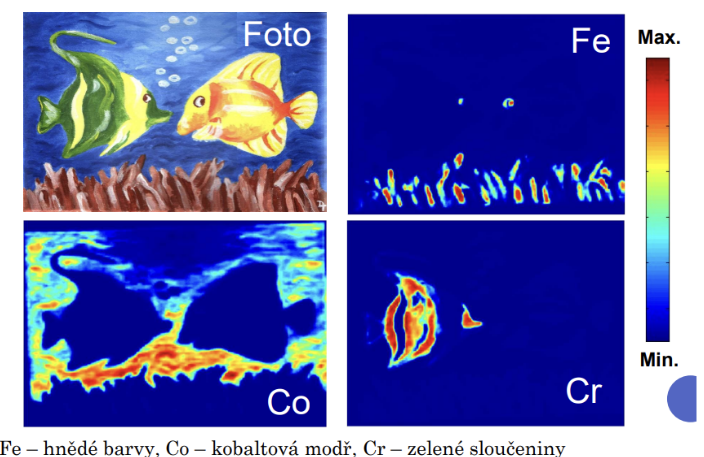
\includegraphics[width=0.6\linewidth]{img/využití elektronové mikrosondy v praxi.png}
    \caption{Využití elektronové mikrosondy v praxi}
\end{figure}

\subsection{Výhody a nevýhody elektronového mikroskopu}

\textbf{Výhody:}
\begin{itemize}
    \item Vysoké rozlišení -- pracují s elektromagnetickými čočkami namísto optickými, což umožňuje dosahovat mnohem vyššího rozlišení než světelné mikroskopy. To je zvláště užitečné při studiu malých struktur na mikro a nano úrovni.
    \item Velké zvětšení -- díky schopnosti pracovat s krátkou vlnovou délkou elektronů mohou elektronové mikroskopy dosáhnout velkých zvětšení.
    \item Podrobný pohled na vnitřní struktury -- TEM umožňuje podrobný pohled na vnitřní struktury vzorků, což je užitečné pro studium buněčné a materiálové biologie.
    \item Trojrozměrný obraz: SEM poskytuje trojrozměrný obraz povrchu vzorku, což je užitečné pro studium morfologie.
    \item Široká škála aplikací - materiálový výzkum, umění, archeologie, částečně i geologie a biologické předměty.
\end{itemize}

\textbf{Nevýhody:}
\begin{itemize}
    \item Vysoké náklady -- elektronové mikroskopy jsou nákladné na pořízení, údržbu a provoz.
    \item Složitá obsluha -- obsluha elektronových mikroskopů vyžaduje odborné znalosti a dovednosti a proto vyžaduje školený personál.
    \item Vakuové prostředí -- pro správnou funkci je nutné pracovat ve vakuovém prostředí, což může omezit studium některých živých vzorků.
    \item Příprava vzorků -- příprava vzorků může být složitá a vyžaduje speciální postupy, jako je například nástřik tenké vrstvy kovu pro TEM.
    \item Rozměry a hmotnost -- elektronové mikroskopy jsou obvykle velké a těžké zařízení, což omezuje jejich přenosnost a umístění do menších laboratoří.
\end{itemize}
\section[Aplikace ionizujícího záření v geologii a geofyzice]{Aplikace ionizujícího záření v geologii a geofyzice}

\subsection{Radiometrické datování hornin}

\textbf{Uran -- olovo:}

= Výhradně pro vulkanické horniny, k datování se používá Zr $\rightarrow$ ZrSiO$_4$.

\begin{itemize}
    \item[1)] Máme zirkon ZrSiO$_4$, který obsahuje malé množství U-238 a U-235.
    \item[2)] Dochází k jejich rozpadu $\rightarrow$ vznik stabilních izotopů olova.
    \item[3)] Zirkon krystalizuje z magmatu $\rightarrow$ silně vytlačuje veškeré olovo -$\rightarrow$ předpoklad: po vyvření není ve vyvřelině žádné olovo $\rightarrow$ uzavřený systém pro U i Pb.    
    \item[4)] Jakékoliv olovo, co je detekováno, poté odpovídá rozpadu uranu (tzv. radiogenní olovo).
    \item[5)] Určí se poměr U/Pb $\rightarrow$ hmotnostní spektrometrie .
\end{itemize}

\textbf{Burial dating method -- Al a Be:}

\begin{itemize}
    \item[1)] Máme kosmogenní izotopy $^{26}$Al a $^{10}$Be -- vznik interakcí kosmického záření -- akumulace v horninách jako křemen
    \item[2)] Vznikne zhrubaa konstantní poměr $^{26}$Al a $^{10}$Be .
    \item[3)] Po pohřbení $\rightarrow$ odstínění od kosmického záření $\rightarrow$ poločas hliníku: 729 000 let, u beryllia: 1,39 milionů let $\rightarrow$ hliník se rozpadá rychleji .
    \item[4)] Z poměru můžu určit stáří.
    \item[5)] Limitace na látky obsahující křemen, stáří v stovkách tisíc až milionech let.
\end{itemize}

\textbf{Letecké monitorování} = spektrometrické měření záření gama ze svrchní vrstvy půdy. Umožňuje získat informace o vlastnostech hornin a půd a zejména o jejich obsahu přírodních radionuklidů (především K, U, Th).

Můžu využít i při vyhledávání ložisek uranu, měření v dolech. Dále lze gamma spektrometrii využít v závodě na zpracování uranu, kde jsou jednotlivé vozíky/haldy uranu rozřazovány podle intenzity záření.

Ve stavebnictví využívám při měření radonu. Ten kromě jiného může být měřen při vyhledávání zlomů v půdě, neboť cestuje vzhůru právě skrz zlomy.

\subsection{Jaderná karotáž (well logging)}

Karotáž je metoda v geofyzice, která se používá k měření fyzikálních vlastností hornin v podzemí, zejména při průzkumu a těžbě ropy a zemního plynu. Radiometrická karotáž je jedním z typů této metody, která využívá radioaktivních vlastností hornin.

Princip spočívá v detekci a měření radioaktivního záření emitovaného horninami. Toto záření pochází z přirozeně se vyskytujících radioaktivních prvků, jako jsou uran, thorium a K-40, které jsou součástí hornin. Tyto prvky emitují gama záření, které lze detekovat a měřit pomocí vhodných detektorů umístěných na vrtacích zařízeních.

Při radiometrické karotáži se na vrtací nástroje (karoty) umístí detektory, které registrují gama záření vysílané z hornin. Intenzita tohoto záření může poskytnout informace o složení hornin. Například vysoký obsah uranu může indikovat přítomnost uranových rud, což může být důležité pro průzkum ložisek uranu.

\textbf{Nuclear borehole logging} (jaderná karotáž) je metoda, která využívá velké prostupnosti neutronů a gama záření. Využívá se v průmyslu pro ropu, zemní plyn a uran. Jedná se o metody, které umožňují detekci nestabilních izotopů, a nebo metody, které takovéto izotopy vytváří, což se pak detekuje. Výhodou je dobrá penetrace záření, díky čemuž záření snadno projde skrze obalové materiály. Tyto metody je možné využívat i pokud je vrt vyplněn kapalinou. 

Metody:

\begin{itemize}
    \item \textbf{Gama karotáž}: Nejvíce využívané, jedná se o pasivní metodu. V zásadě jen přijímáme měření. Nejčastější aplikace je v lithologii (nauka o výzkumu a popisu usazených hornin) a v stratigrafii (určování stáří hornin). Zaznamenává se celkové gama záření detekované ve vrtu, neboli expoziční příkon v hornině, či stanovení obsahu jednotlivých radioaktivních prvků v rudním průzkumu. 
    
    Hlavní radioizotopy: thorium (Th-230 a Th-232), draslík (K-40) a uran (U-235 a U-238).
    
    Pokud signál je zesílený $\rightarrow$ asi břidlice, pokud zeslabený $\rightarrow$ pískovec, vápenec, dolomit -- můžu mít ještě spektrální gamma karotáž, čímž stanovím obsah radioaktivních prvků ve vrtu.

    \item \textbf{Gama-Gama karotáž}: Jedná se o aktivní metodu, kde je potřeba učinit nějakou "akci". Gama záření je vyzářeno ze zdroje v zavedené sondě ve vrtu. Toto záření pak prochází okolníma šutrama, interaguje, a pomocí Comptonova rozptylu je zpětně detekováno v detektorech, které se taktéž nachází v zavážené sondě. Výsledkem je stanovení hustoty, pórovitosti atd.
    
    Platí totiž, že odezva bude nepřímo úměrná elektronové hustotě. Detektor v karotážní sondě měří intenzitu gama záření, které se vrací k sondě po interakci s horninou. Nižší intenzita detekovaného záření indikuje vyšší hustotu horniny, protože více záření bylo rozptýleno nebo absorbováno. Naopak vyšší intenzita naznačuje nižší hustotu horniny. 
    
    Druhá možná varianta je detekce sekundárního záření vzniklé fotoefektem, čímž se stanovuje obsah těžkých prvků jako Ba, Sb, Pb. Zdrojem gama záření je často Cs-137. Detektory jsou vhodně odstíněny od zářiče.

    \item \textbf{Neutronová karotáź}: Obsahuje neutronový zdroj v zavedené sondě a detektory pro záznam interakcí, ke kterým dochází v blízkosti vrtu, do kterého je sonda zavedená. Emitované vysokoenergetické neutrony jsou postupně zpomalovány (nejvíce na jádrech vodíku) a následně mohou být absorbovány v materiálu a nebo v detektoru neutronů. Proto lze hovořit o \textbf{neutron-gama karotáži} (měřím charakteristické gamma vzniklé při interakci neutronu s horninou) a o \textbf{neutron-neutron karotáži}, kdy detekuji zpomalené tepelné neutrony, které difundovaly až k detektoru. Většina těchto interakcí závisí na množství přítomného vodíku, a tedy i vody v šutrácích, které jsme provrtali při vrtání vrtu. Nejčastější zdroj vysokoenergetických neutronů je AmBe.

    Neutronová karotáž je obecně souhrn pro neutron-neutron karotáž (zdroj rychlých neutronů $\rightarrow$ zpomalení v hornině $\rightarrow$ stanovení pórovitosti hornin (zpomalení na vodíku)). Dále sem patří neutron-gama karotáž (radiační záchyt neutronů, stanovení pórovitosti, rozhraní plyn-ropa a plyn-voda a také některých prvků Cl, Ni, Fe, Cu, Ti, Mn) a na závěr sem patří Neutronová aktivační karotáž (v podstatě aktivační analýza a měříme charakteristické záření vzniklého radioaktivního izotopu $\rightarrow$ stanovení Cu, Mn, Al, Si, F).
    
% V geologickém průzkumu se už dávno využívá tzv. radioaktivní karotáž. při ní se do geologického vrtu nejprve spustí
% sonda s neutronovým zářičem a poté se měří sekundární radioaktivita geologických vrstev, vyvolaná tokem neutronů.
% Měřením aktivity plynných radionuklidů v půdě se určuje stáří geologických vrstev, rozptylem neutronů se měří vlhkost
% půdy nebo přítomnost zdrojů podzemní vody či ropy

\end{itemize}

Vodohospodáři využívají radionuklidy k měření průtoků v řekách i vodovodních potrubích. Do vody nebo vodního toku je vstříknut radioizotop (bez zátěže ŽP) a následně je tento izotop detekován v místě s různými detektory (můžou být různě podél břehu i v hloubce). Na základě času a koncentrace lze stanovit průtok. Používám, když nemohu použít standardní metody. 

Rozlišuji:

\begin{itemize}
    \item metodu časové distribuce -- sleduji za jak dlouho se mi vzorek dopravil z bodu A do bodu B a v jaké koncentraci,
    \item metodu ředění -- podle toho, jak se koncentrace v toku mění, určím průtok.
\end{itemize}

Ozařováním je možno ošetřit také odpadní vody obsahující některé nebezpečné látky ještě před přivedením do běžných čističek odpadních vod. Zářiče s radiokobaltem zabraňují množení nežádoucích mikroorganizmů, které snižují kvalitu pitné vody ve studních.

\begin{figure}[H]
    \centering
    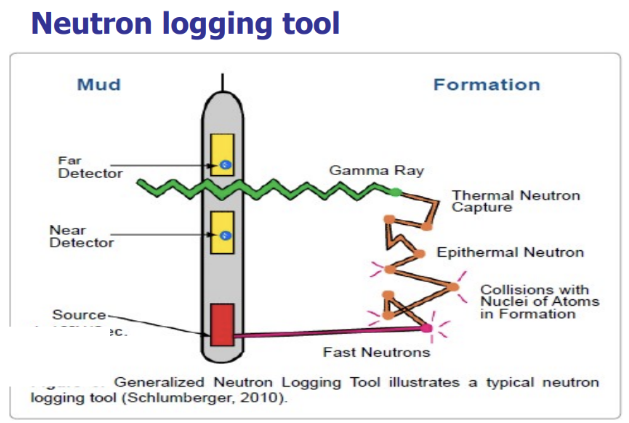
\includegraphics[width=0.8\linewidth]{img/Neutronová karotáž.png}
    \caption{Neutronová karotáž}
\end{figure}

\subsection{Metody využívající zpětný odraz gama}

\textbf{Stanovení obsahu popela v uhlí:}

Zpětný rozptyl záření gama se například využívá pro stanovení obsahu popela v uhlí, kde využívá energetické závislosti píku zpětně odraženého gama záření. Princip je vlastně identický jako u gamma-gamma karotáže:

\begin{itemize}
    \item[1)] Emitované fotony interagují s materiálem (uhlí) $\rightarrow$ Comptonův rozptyl, část fotonů odražena zpět.
    \item[2)] Detektorem měřím intenzitu odražených fotonů.
    \item[3)] Míra rozptylu závisí na hustotě elektronů v materiálu, což je ovlivněno atomovým složením a hustotou.
    \item[-] uhlí -- především H, C, O, N a S \& popel $\rightarrow$ těžší sloučeniny -- oxidy křemíku, hliníku, železa, vápníku etc.
    \item[-] popel -- větší $Z$ $\rightarrow$ více elektronů \& větší hustota $\rightarrow$ větší elektronová hustota $\rightarrow$ pravděpodobnější rozptyl a absorpce $\rightarrow$ pokles intenzity.
    \item[4)] Naopak tam, kde je hodně uhlí a málo popela $\rightarrow$ vysoká intenzita odraženého gamma.
\end{itemize}

Řízení přívodu uhlí do elektrárny:

\begin{itemize}
     \item Provoz elektrárny vyžaduje přívod uhlí o specifické výhřevnosti. V případě jakékoliv odchylky může dojít ke ztrátě výkonu nebo dokonce k výpadku kotle.
     \item Obsah popela uhelného uhlí a výhřevnost je sledována před plněním sila, aby byla zajištěna dostatečná kvalita uhlí pro správný provoz kotle.
     \item  V případě, že on-line bilance kvality uhlí neodpovídají požadavkům kotle, lze do některých sil nakládat uhlí různé kvality.
    \item  Parametry veškerého uhlí, které je pro kotel k dispozici, slouží obsluze k úpravě pracovních parametrů kotle podle potřeby.
\end{itemize}

\textbf{In-situ analýza a kontrola těžby:}

V některých případech je možné gamma záření využít pro in-situ analýzu hornin během těžby. Speciální zařízení mohou měřit intenzitu gamma záření přímo na místě a poskytovat okamžitou zpětnou vazbu o kvalitě rudy. To umožňuje optimalizovat proces těžby a zpracování nerostů tím, že těžba může být řízena na základě skutečné kvality vytěženého materiálu.

\begin{itemize}
    \item In-situ leaching: roztok kyseliny rozpouští uran z rudy $\rightarrow$ následně je monitorována koncentrace uranu v roztoku, optimalizováno pro co nejmenší dopasd na ŽP a efektivnost práce.
    \item Lze také při klasické těžbě - monitoruji jednotlivé "vozíky" s rudou.
\end{itemize}

%Nejsem si jistý, jestli se měří radiaktivní izotopy (uran, thorium ...) -- tzn. pasivní metoda, nebo se sleduje také rozptyl (nebo charakteristické záření?) asi by šlo sestrojit různé metody.

Pásová analýza (nebo-li analýza materiálu v průběhu toho co mi běží na běžícím páse a mohu tak online stanovovat kvalitu uhlí): Metoda stanovení obsahu popela v uhlí pomocí gama záření využívá principu měření intenzity gama záření, které prochází vzorkem uhlí. Popel v uhlí má specifické vlastnosti, které ovlivňují absorpci a rozptyl gama záření. Na základě těchto změn lze určit obsah popela ve vzorku.

\textbf{Analýza kalů (slurry analysis):} 

Gama záření se používá k měření koncentrace pevných částic v kalu. Princip je podobný jako u měření obsahu popela v uhlí či stanovování hustoty, ale také se využívá při loggingu (karotáž, viz Vrtání do země, psáno výše).

\underline{Pozn.:} Jak odhalím podíl prvku ve sloučenině? Pokud je prvek dostatečně těžký, resp. všechny prvky, co jsou ve sloučenině, není nic jednoduššího než použít RFA a využít detekci charakteristického RTG záření. Pokud je ovšem třeba jen jeden prvek ze dvou, tak to jde taky tak udělat a od celkového množství odečtu to, co naměřím, čímž získám zbytek. Možností je také využít rozdílu mezi fotoefektem a comptonovým roztpylem, kde fotoefekt má vyšší pravděpodobnost pro těžší atomy, a proto se na celkovém podílu reakcí více podílí pro lehké atomy Comptonovův rozptyl. Poslední možností je, pokud to umožňuje, využít neutronovou aktivační analýzu.
\section[Využití iontových svazků v materiálovém výzkumu]{Využití iontových svazků v materiálovém výzkumu: Základní typy urychlovačů, Metody RBS, kanálování, PIXE, PIGE, ERDA a NRA}

\subsection{Základní typy urychlovačů}

\textbf{Definice:} Urychlovač je zařízení, které umožňuje zvýšení kinetické energie nabité (urychlované) částice, a to pomocí elektrické pole, které může být statické nebo proměnně a přitom je vede po stanovené trajektorii, a to pomocí megnetického pole, jež může být opět statické a nebo proměnné. Urychlovat lze pouze nabité částice, stejně tak jako je vést po určité dráze vlivem magnetického/elektromagnetického pole.

Díky případnému konverznímu materiálu lze eventuelně převést nabité částice na jiný typ záření (neutrony, fotony).

\textbf{Základní komponenty urychlovače:}

\begin{itemize}
    \item Zdroj nabitých částic
    \item Urychlovací trubice (EM pole)
    \begin{itemize}
        \item VN zdroj vytvářecí urychlovací napětí a magnety v urychlovačí (dipóly = zakřivení dráhy pohybu částic, kvadrupóly = fokusace svazku).
    \end{itemize}
    \item Systém dodávky EM polí
    \item Extrakce urychlených částic z urychlovače a soustředění na terčík
    \item Bombardovaný terčík a detektor/y pro popis parametrů urychleného svazku
    \item Diagnostika svazku (sledování energie, intenzity, polohy)
    \item Systém napájení
    \item Řídicí systém
    \item Vakuový systém
\end{itemize}

\textbf{Rozdělení:}

\begin{itemize}
    \item Dle trajektorie -- Dle trajektorie rozdělujeme urychlovače na lineární (elektrostatické vs. rezonanční, pro konstantní vs. proměnné urychlovací napětí) a cyklické (mikrotron, betatron, cyklotron, synchrotron, synchocyklotron, izochronní cyklotron).
    \item Dle způsobu urychlení -- Dle způsobu urychlení rozdělujeme Elektrostatické a Rezonanční, což je například pro lineární urychlovače velmi efektivní a jsme schopni získat jednotky až desítky MeV na jednotkách metrů (1 m je cca jednotky až destíky MeV).
    \item Dle režimu práce -- Kontinuální (časově neměnný svazek) a Impulzní (uvolňování částic po částech/balících).
\end{itemize}

\textbf{Princip urychlení a zakřivení}:

Velmi to záleží jestli mám cyklický a nebo lineární a pak podle typu napětí EM pole.

\begin{itemize}
    \item Lineární elektrostatický $\rightarrow$ v tomto případě mám rovnou trubici, kde mám dáno urychlovací napětí konstatní a částice je na dáne dráze urychlena tak moc, jak je dáno napětí. Magnetické pole pak zde slouží v podobě dipólů nebo kvadrupólů, a to pro korekci svazku, aby se nevychyloval a pro jeho fokusaci. K tomu se pak typicky ale využívá tzv. elektrostatický fokusační systém, který je tvořen 4 elektrodami, jež jsou vždy 2 a 2 naproti sobě se stejným napětím a způsobují, že částice je "odrážena" doprostřed.
    \item Lineární rezonanční $\rightarrow$ Přímočará dráha pohybum proměnlivý proud (napětí se cyklicky mění a jednotlivé elektrody mění náboj, aby buď odpuzovaly či přitahovaly), zvětšující se délka urychlovacích segmentů s délkou (částice se hýbe velmi rychle, tak to musí mít nějaký efekt a aby ji to vůbec stihlo urychlit, tak jsou delší a delší). Hodně se to využívá v medicíně, protože na krátké vzdálenosti naberou částice vysokou energii a poté se využívá např. převod elektronu na RTG či $\gamma$. V klidu se dá urychlit na 10-15 MeV/m
    \item Cyklický (konst. napětí i magnetické pole) $\rightarrow$ V tomto případě přiletí částice a urychlovacím napětím jí roste energie a magnetickým polem je zakřivena její dráha pohybu, která se s jeho konstatností zvětšuje v poloměru. Celý urychlovač je navržen tak, že při správné energii dosáhne částice maximálního poloměru dráhy pohybu a vyletí ústím ven.
    \item Cyklický (konst. napětí) $\rightarrow$ Stejné jako výše, avšak pomocí proměnlivého magnetického pole mohu částici udržovat na stejném poloměru zakřivení.
    \item Cyklický (obojí proměnlivé) $\rightarrow$ Mám tam například místa, kde když částice projde, tak ji to urychlý a stejně jako u lineárního dochází k periodickému přepólování, aby částice byla odpuzována/přitahována ve správný moment. Proměnlivým magnetickým polem je pak držena na stejném poloměru.
\end{itemize}

\textbf{Využití:} Materiálový výzkum, částicová fyzika, Produkce radionuklidů (do medicíny či materiálový výzkum), Produkce neutronů (studium radiačního poškození, difrakce neutronů, neutronová fyzika, produkce fotonů (materiálový výzkum-XFEL a medicína).

\subsection{Metoda RBS}

= Rutherford Backscatterring Spectroscopy

Využití pružného rozptylu nalétávajících iontů z monoenergetického svazku (E=1-3 MeV) s atomy či jejich elektrony v terčíku.

\begin{itemize}
    \item Pružný rozptyl = bez ztráty energie na srážku
    \item Měření počtu a energii odražených iontů dopadajícího svazku, což nám dává info o materiálu terčíku.
    \item Typické hloubky, kde je RBS schopno identifikovat a lokalizovat různé prvky v matrici jsou desítky až stovky nm.
\end{itemize}

\textbf{Výhody:}

\begin{itemize}
\item vysoká citlivost na těžké prvky v lehké matrici
\item jednoduché umístění vzorku na vzduchu
\item kvalitativní přesnost < 1 \%
\item hloubkové rozlišení < 5 nm se Si(Li) detektorem
\item kanálování
\item Vysoká přesnost na těžké prvky v lehké matrici
\item Schopnost velmi dobře rozlišit dva lehké prvky mezi sebou navzájem (dva lehké prvky s malým rozdílem hmotnosti), a to např. O-18 a F-19, C-13 a N-14
\end{itemize}

\textbf{Nevýhody:}

\begin{itemize}
\item necitlivé na lehké prvky v těžké matrici
\item implantování iontů do analyzovaného materiálu
\item potřebný urychlovač
\item Problém rozlišit dva těžké prvky o podobné hmotnosti (Pb-208 a Au-197), avšak rozlišovací schopnost lze zlepšit zvýšením hmotnosti dopadající částice ($M_1$) $~rightarrow$ citlivost při dopadu alfa částice je lepší v porovnání s protony.
\end{itemize}

\begin{figure}[H]
    \centering
	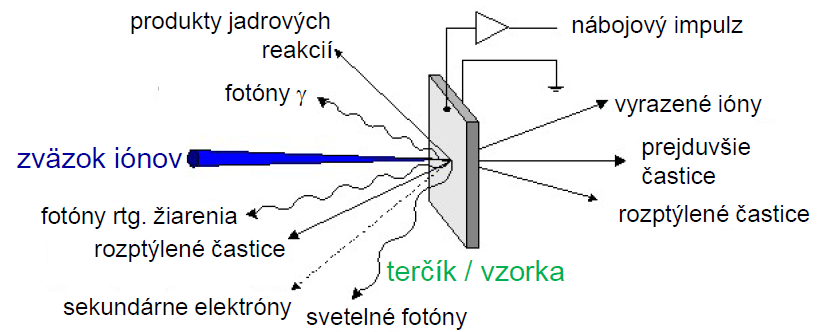
\includegraphics[width=10cm]{img/iont-svazky.png}
	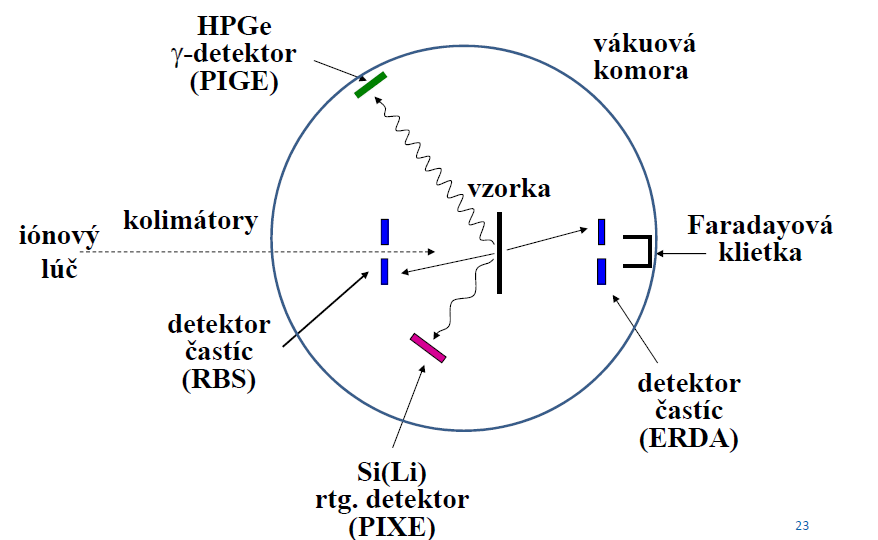
\includegraphics[width=7cm]{img/iont-svazky-exp.png}
\end{figure}

V zásadě existují dva procesy, resp. interakce urychlených iontů s danou látkou:

\textbf{1) Interakce s jádrem (Elastický Coulombův rozptyl):}

\begin{itemize}
    \item Víme počáteční energii $E_0$, víme jeho hmotnost $M_1$ a měříme jeho energii $E_1$ po jeho zpětném rozptylu.
    \item Využijeme $E_1$ = K * $E_0$, kde K je kinematický faktor a je funkcí hmotností obou interagujících částic a úhlu odrazu zaznamenáného odraženého iontu
    \item Neznámou tedy představuje pouze hmotnost $M_2$, kterou jsme schopni z toho dopočítat a určit o jaké jádro se jedná.
\end{itemize}

\textbf{2) Interakce s elektrony (elektronový rozptyl):}

\begin{itemize}
    \item Lokalizace a určení atomu ($M_2$) jakožto funkce hloubky, resp. v závislosti na tom v jaké hloubce dojde k rozptylu.
    \item množství úbytku energie záleží na brzdném účinku látky, tedy na hustotě elektronů v látce a vzdálenosti, kterou nabitý iont urazí při průchodu látkou.
    \item Prvky, které se v materiálu objevují pouze v určité hloubce mají na naměřeném spektru svůj pík posunuty, ale jsou posunuty o jistou míru/energii, která představuje vzdálenost, kterou musel iont projít materiálem, aby se k nim dostal.
    \item Ke stanovení je nutné mít naměřenou energii iontu po odrazu na povrchu a pak následně v dané hloubce. Čím hlouběji iont musel jít, tím více ztratí energie
    \item Správnost určení rozdílu energií při odrazu na povrchu a v hloubce ($\Delta E$) závisí na = energetické rozlišení detektoru, energetický rozptyl urychleného svazku dopadajících iontů a také energetický rozptyl směrem k a od terčíku, příprava povrchu terčíku. Na závěr samozřejmě závisí na materiálu, který je měřen.
\end{itemize}

\textbf{Měřené spektrum podle tloušťky měřeného vzorku materiálu:}

\begin{itemize}
    \item Ultra tenká vrstva (několik atomárních vrstev)
    \begin{figure}[H]
        \centering
        \includegraphics[width=0.5\linewidth]{img/ultra tenká vrstva - RBS.png}
        \caption{ultra tenká vrstva -- RBS}
    \end{figure}

    \item Tenká vrstva (několik stovek až tisíců atomárních vrstev)

    \begin{figure}[H]
        \centering
        \includegraphics[width=0.5\linewidth]{img/Tenká vrstva - RBS.png}
        \caption{Tenká vrstva -- RBS}
    \end{figure}

    \item Hrubá vrstva = toto už jsou mm, v zásadě bulk/objem.

    \begin{figure}[H]
        \centering
        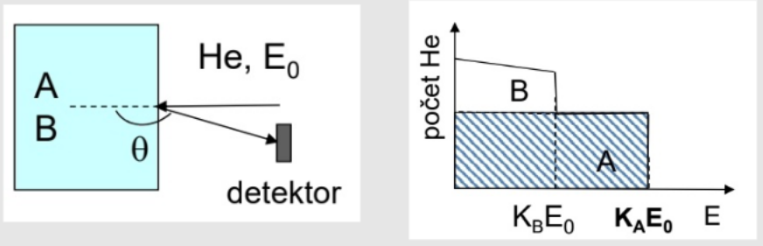
\includegraphics[width=0.5\linewidth]{img/Bulk - RBS.png}
        \caption{Bulk -- RBS}
    \end{figure}

    \item Pokrytí povrchu = bulk materiál, který má na povrchu naneseny různé tloušťky jiného materiálu/materiálů. Zde rozdělujeme 2 varianty (lehký bulk a těžké pokrytí a naopak)

    \begin{figure}[H]
        \centering
        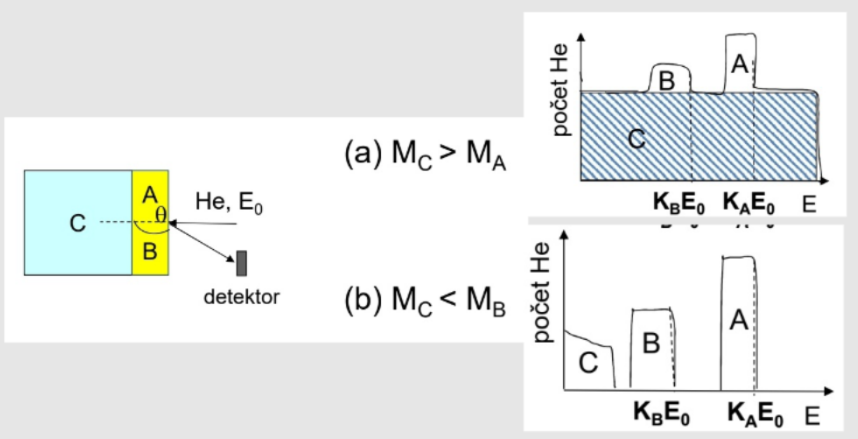
\includegraphics[width=0.5\linewidth]{img/pokrytí - RBS.png}
        \caption{Pokrytí -- RBS}
    \end{figure}
\end{itemize}

\textbf{Kvalitativní analýza:}

\begin{figure}[H]
    \centering
	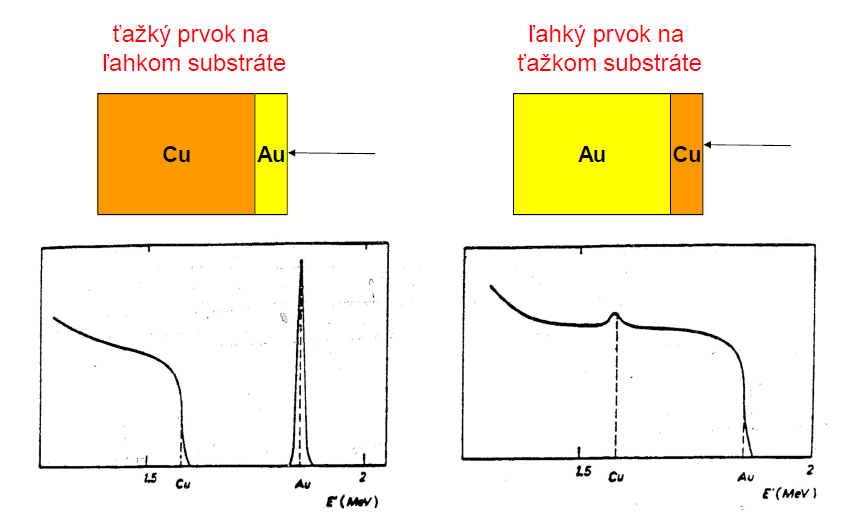
\includegraphics[width=9cm]{img/rbs-analyza.png}
	%	\includegraphics[width=7cm]{rbs2.png}
	%	\includegraphics[width=7cm]{rbs3.png}
\end{figure}

Výstupem při měření dostáváme z detektoru impulsy, jejichž výška je úměrná energii zpětně odraženého iontu. Z výšky čar výsledného spektra lze stanovit stechiometrické složení vzorku.

\textbf{Využití:}

Detektory částic nastavené na RBS jsou často součásti většího celku jehož součásti jsou i detektory na PIGE, PIXE, ERDA a celé to bývá vaukováno, aby nedocházelo k parazitní interakci s částicemi atmosféry (nahoře je ovšem psáno, že RBS jde dělat i na vzduchu, což jde, ale je lepší tam tu parazitní interakci nemít).

Umění, archeologie (sochy, obrazy, předměty -- například rozdíl mezi zlatem a pozlacením), materiálový výzkum a geologie.

\subsection{Kanálování}

Kanálování je speciální mód RBS techniky. Vyžadováno je, aby orientace urychlených iontů byla ve správné poloze vůči krystalografické mříži, a to konkrétně podél hlavní krystalografické osy krystalu.

V čistém a ideálním krystalu by měl iont jakoby "projít rovně skrz  a mezi jednotlivými rovinami", avšak v případě přítomnosti poruch či příměsí jsme schopni detekovat jejich polohu v krystalu, jelikož pak dochází k poklesu intenzity detekovaného záření (stínení Coulombovského rozptylu).

\begin{figure}[H]
    \centering
	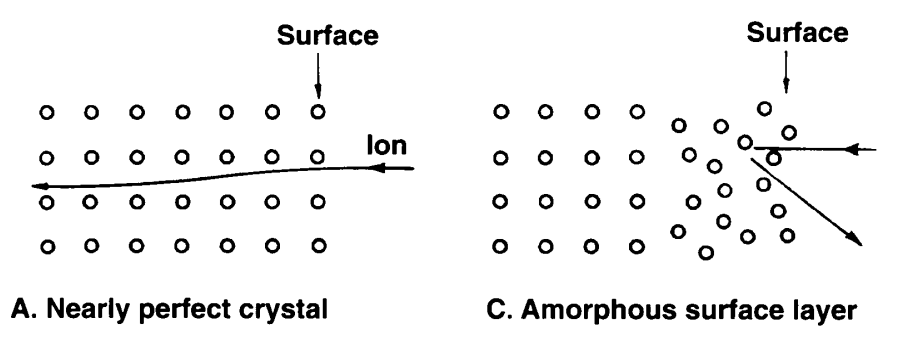
\includegraphics[width=10cm]{img/rbs-kanalovani.png}
	%	\includegraphics[width=7cm]{rbs2.png}
	%	\includegraphics[width=7cm]{rbs3.png}
\end{figure}

\subsection{PIXE}

= Particle Induced X-Ray Emission

Jedná se nedestruktivní o metodu, která využívá detekce charakteristického RTG záření.

\textbf{Výhody:}

\begin{itemize}
    \item Nedestruktivní technika schopna měřit tuhé látky, tekutiny i aerosoly
    \item Vysoká citlivost a rychlost měření
    \item Dobrá rozlišovací schopnost = multiprvková analýza (Z > 13 = Al)
\end{itemize}

\textbf{Nevýhody:}

\begin{itemize}
    \item Nelze analyzovat organické vzorky
    \item Omezená hloubková informace
    \item Potřeba urychlovače
\end{itemize}

\textbf{Princip:}

Excitací atomu iontovým svazkem (vyražení elektronu a jeho zabrání elektronem z vyšší energetické hladiny) a produkce charakteristického RTG záření, jehož detekči lze identifikovat původce a identifikovat tak prvek (v zásadě stejné jako u RFA, akorát tady se využívají ionty a ne fotony z radionuklidu nebo rentgenky).

Stejně jako u RFA, tak i zde je Augerův elektron konkurenční jev a dohromady dávají jedničku. Takže existuje klasicky pravděpodobnost, že k vyzáření RTG dojde a ta je dána účinným průřezem pro ionizaci a fluorescenčním výtěžkem.

Stejně jako u RFA, tak se projevují matricové jevy, které mi ovlivňují měření, tedy to co naměřím a to co realně je ve zkoumaném materiálu.

Stejně jako u RFA, tak plocha pod čarou je rovna koncentraci prvku

K detekci charakteristického RTG záření se využívá HPGe, Si(Li)

\begin{figure}[H]
    \centering
	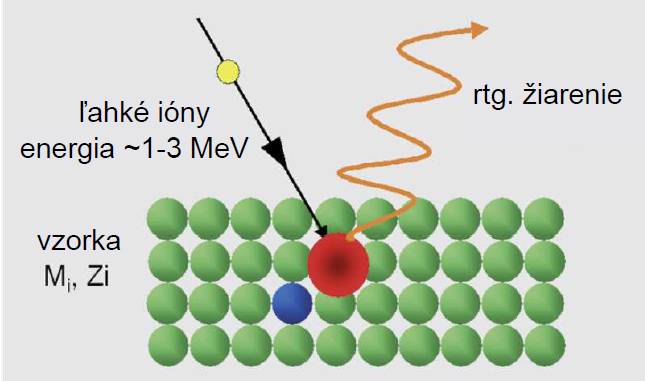
\includegraphics[width=8cm]{img/pixe.png}
	%	\includegraphics[width=7cm]{rbs2.png}
	%	\includegraphics[width=7cm]{rbs3.png}
\end{figure}

\textbf{Aplikace a využití:}

\begin{itemize}
    \item Materiálový výzkum
    \item Geologie
    \item Umění, architektura
    \item Monitoring znečištění atmosfŕy
\end{itemize}

\textbf{Speciální případy:}

\begin{itemize}
    \item Mikrosvazek = distribuce prvků ve vzorku (analýza hrubých vrstve s vysokým rozlišením) $\rightarrow$ stopová množství, malé oblasti s vysokým rozlišením.
    \item Externí svazek = Analýza velkých a komplexních předmětů svazkem z urychlovače, který je vyveden ven do atmosféry na zkoumaný objekt (proto externí svazek)$\rightarrow$ Louvre, artefakty, obrazy.
\end{itemize}

\subsection{PIGE}

=Particle Induced Gamma Emission

Jedná se o nedestruktivní metodu pro stanovení prvkového složení na základě interakce urychlených protonů, popř. d, $\alpha$ a málokdy těžkých iontů s jádrem atomu za vzniku gama záření, které poté detekujeme. Toto záření tak je pak v některých případech doprovázeno ještě další reakcí, resp. vznikem další částice/záření.

Nejčastěji se opět měří ve vakuové komoře a nejvíce se využívají urychlené protony.

\begin{itemize}
    \item Rezonanční záchyt (p, $\gamma$) - mohu využít rezonancí prvků, které jsou ve zkoumaném materiálu a pak detekuji jen gamu. To ale vyžaduje, že vím co tam je, resp. vím co v tom hledám, abych danou rezonanci mohl využít.
    \item nepružný záchyt (p, $p^| \gamma$)
    \item Srážky s přeuspořádáním (p, n$\gamma$), (p, $\alpha\gamma$), (p,n)
\end{itemize}

\subsection{ERDA}

=Elastic Recoil Detection Analysis

Jedná se o metodu využívající pružný rozptyl lehkých jader po dopadu těžkých iontů. Slouží pro detekci lehkých prvků v těžké matrici (dokáže detekovat vodík v tuhých látkách)

\textbf{Výhody:}

\begin{itemize}
    \item Dobrá citlivost na lehké prvky.
    \item Dá se kombinovat s RBS.
    \item Menší poškození vyšetřovaného materiálu.
    \item Idektifikace 1-H a 2-H hloubkových profilů (pomocí alfa).
\end{itemize}

\textbf{Nevýhody:}

\begin{itemize}
    \item Menší hloubkové rozlišení a hloubka analýzy (způsobeno hmotností, resp. velikosti těžších iontů) je kvůli rozptylu dopadajících iontů asi několik stovek nm.
    \item Vzorek musí být spešl připraven + omezená geometrie ozařování a detekce.
\end{itemize}

\textbf{Princip:}

Pružný rozptyl dopadajícíh vysokoenergetických a těžkých iontů (MeV), ven jdou odražené ionty a vyražené atomy z materiálu

Umožňuje profilování lehkých jader.

S využitím standardů umožňuje i kvantitativní analýzu.

\begin{figure}[H]
    \centering
	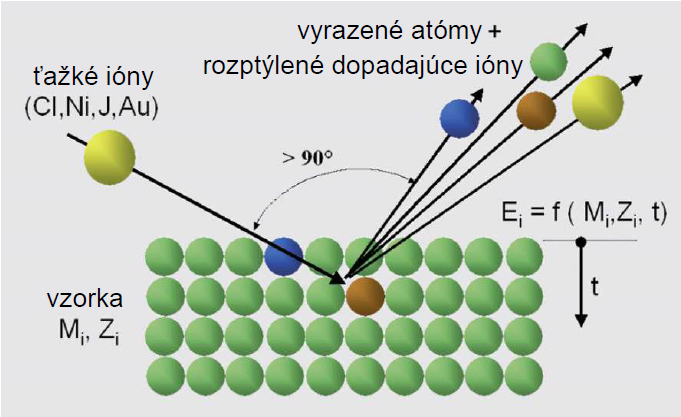
\includegraphics[width=8cm]{img/erda.png}
	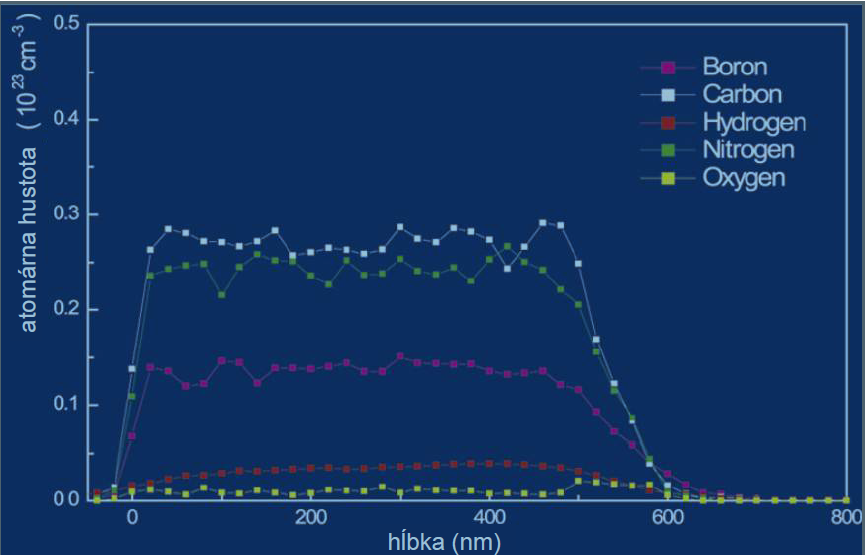
\includegraphics[width=7cm]{img/erda-spektrum.png}
	%	\includegraphics[width=7cm]{rbs3.png}
\end{figure}

\textbf{Módy provozu:}

\begin{itemize}
    \item Transmisní: Velmi tenké vzorky
    
    \begin{figure}[H]
        \centering
        \includegraphics[width=0.38\linewidth]{img/transmisní ERDA.png}
        \caption{transmisní ERDA}
    \end{figure}

    \item Odraz pod malými úhly = nejčastější metoda

    \begin{figure}[H]
        \centering
        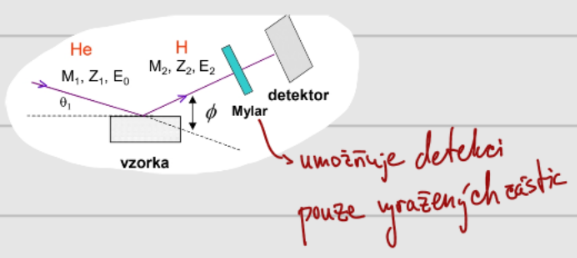
\includegraphics[width=0.5\linewidth]{img/odrazová ERDA.png}
        \caption{odrazová ERDA}
    \end{figure}
\end{itemize}

V obou geometriích platí, že $E_2 = K * E_0$, kde faktor $K$ závisí na hmotnostech bombradující a vyražené částice a dále na úhlu rozptylum takže pak jen určíme zase hmotnost $M_2$.

\subsection{NRA}

= Nuclear Reaction Analysis

Jedná se o metodu pro detekci lehkých prvků (Z < 18), jež je izotopicky citlivá a umožňuje identifikaci a lokalizaci stopových prvků. Jedná se o nedestruktivní metodu s analytickou hloubkou několik stovek nm, ovšem jedná se vždy o exotermickou nebo endotermickou reakci a tudíž energetická bilance je vždy nenulová.

Jedná se o nepružný proces, a proto se částice na začátku nerovnají produktům reakce.

\textbf{Princip:}

Jaderná reakce mezi dopadajícím iontem a prvkami v terčíku. Následně dochází k detekci produktů reakce ($\gamma$ nebo částice).

\begin{figure}[H]
    \centering
	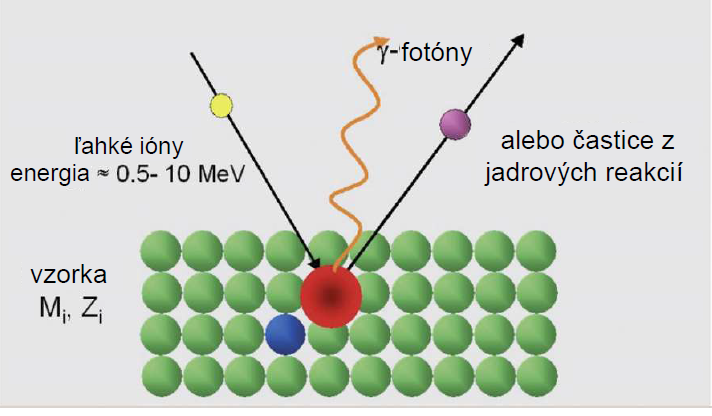
\includegraphics[width=8cm]{img/nra.png}
	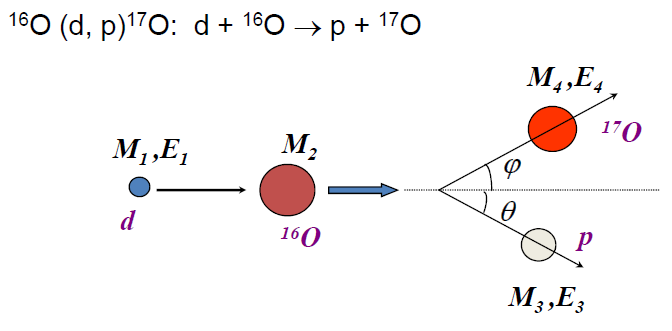
\includegraphics[width=7cm]{img/nra2.png}
	%	\includegraphics[width=7cm]{rbs3.png}
\end{figure}

Detekuji produkty reakce (částice nebo $\gamma$)( pomocí Si detektoru nebo $\gamma$ fotony detekuju pomocí Ge či NaI(Tl) detektorů)a změřím si energii $E_3$ pro dané $M_1$, $E_1$ a $\theta$ a tím identifikuji $M_2$.

Poté si naměřím spektrum $E_3$, které mi podá informaci o hloubkovém rozložení $M_2$ a tím ho lokalizuji v materiálu.


\textbf{Pozn.:} Reakce může probíhat dvojím způsobem, a to sice přes složené jádro (všechny nukleony jsou využity) a nebo jakožto tzv. přímá reakce, kde jen některé nukleony jsou použité (někdy nazýváno trhací reakce).

Pravděpodobnost reakce je klasicky dána příslušným účinným průřezem.

K detekci příslušných jader v hloubce nebo na povrchu se dají využít rezonance, kdy pokud se energie bombardující částice rovná energii rezonance, tak k interakci dojde na povrchu. Pokud je ovšem energie částice vyšší než energie rezonance, tak k interakci dojde v hloubce pod povrchem (cestou do materiálu se energie sníží a až se vyrovná tak interaguje).

Příkladem je analýza vodíku pomocí 15-N za vzniku 12-C + 4-He a $\gamma$. Rezonance je při 6,385 MeV a s hloubkou dochází k posuvu rezonance, a proto se vyuźívájí energie vyšší než rezonance až napŕ. do 15 MeV.

\textbf{Využití:} Farmacie, archeologie, Geovědy, umění

\textbf{Srovnání RBS a NRA:}

\begin{itemize}
    \item RBS je pro detekci těžkých prvků v lehké matrici, zatímco NRA je pro detekci lehkých prvků.
    \item RBS využívá elastický rozptyl dopadajících částic (typicky $\alpha$ = 2 MeV), zatímco NRA vyuźívá nepružný roztpyl mezi dopadající částicí a částicí v terčíku (detekce produktů reakce)
    \item RBS má energetickou bilanci nulovou a NRA nemá
    \item u RBS jsou jádra terčíku i dopadající částice v základním stavu, zatímco u NRA jsou produkty reakce odlišné od původních, které do reakce vstupují.
\end{itemize}
\section[Využití jaderně-fyzikálních metod v materiálovém výzkumu]{Využití jaderně-fyzikálních metod v materiálovém výzkumu: Mössbauerova spektrometrie, elektron-pozitronová anihilační spektroskopie, neutronová aktivační analýza}

\subsection{Mossbauerova spektrometrie}

Byla objevena německým fyzikem Rudolfem Mossbauerem v roce 1958. Je založeno na rezonanční fluorescenci $\gamma$ záření

Obvykle používané prvky: $^{57}$Fe, $^{119}$Sn, $^{121}$Sb, $^{129}$I.

Široká škála aplikací při studiu chemických vazeb, anorganické chemii pevných látek, atd. Hlavní množství článků a studií je ale zaměřeno na železo.

Jedná se o metodu izotopicky citlivou (bezodrazová jaderná rezonanční absorpce/fluorescence gama záření).

\subsubsection{Princip}

Mossbauerův jev = bezodrazová jaderná rezonanční absorpce gamma záření

\begin{itemize}
    \item Založeno na emisi a absorpci $\gamma$ záření emitovaného jádrem bez zpětného rázu.
    \item Atomy ve zdroji emitující $\gamma$ záření musí být stejné, jako v atomy ve vzorku.
    \item Vlastně je to tak, že jádra ve vzorku jsou excitovaná gammou, která je emitovaná při stejné deexcitaci ve zdroji.
    \item Zde zdroje fotnů jsou generovány fotony o dané energii a pokud je tato energie veeeelmi přesná jako je energie mezi vzbuzeným a základním stavem atomu či jádra ve zkoumaném materiálu, tak dojde k tzv. rezonanční absorpci.
    \item Poté dochází opět k přechodu zkoumaného jádra do základního stavu emisí fotonu o té samé energii, co to původně vyvolala
    \item Celé co chceme je dosáhnout překrycu emisní a absoprpční čáry, což je velmi složité neboť je šířka píku (energie) velmi malá a komplikuje to celé jev tzv. zpětného rázu.
\end{itemize}

\subsubsection{Zpětný ráz}
\begin{itemize}

\item Při emisi vysokoenergetické částice z jádra funguje zpětný odraz, část hybnosti je předaná emitujícímu jádru (analogicky u zbraně -- taky mě to hodí trochu dozadu).
\item Energie gamma záření má proto o trošku nižší energii než je energie rezonance, a to o energii tohoto zpětného rázu.
\item Pro energii zpětného rázu platí: $E_{R} = \dfrac{E_{\gamma}}{2 M c^2}$, kde $M$ je hmotnost emitujícího jádra a $E_{\gamma}$ je energie emitovaného fotonu.
\item S narůstající hmotností $M$ klesá energie zpětného odrazu, a proto platí, že jeli energie emitovaného gama záření malá oproti hmotnosti jádra, jež jej emituje, pak se energie zpětného rázu pohltí a s jádrem to nehne. V opačném případě je třeba tuto energii nějak zohlednit a ideálně ji kompenzovat.
\item V případě nevázaného jádra je posun energie značný a není možné Mossbauerův jev pozorovat. Neboli nedojde k překryvu emisní a absorpční čáry.

Příkladem je známé železo Fe-57 u něhož je šířka čáry 4,6 neV a energie zpětného rázu je 2meV. To znamená, že emitované gama o velikosti 14.4 keV, které na něj letí s cílem ho excitovat, tak mi je k ničemu, protože energie fotonu je nižší o ty 2 meV a tudíž nedosáhnu překryvu emisní a absorpční čáry, která je ultra tenounká. Nutno dále zmínit, že o energii zpětného rázu se mi navíc posouvá nejen emisní čára, ale i absorpční čára, neboť to má vliv i na jádro, jež energii přijíma. Souhrně řečeno: U volného jádra (plynné či kapalné médium) dochází při emisi k zpětnému rázu, o který se sníží energie emitovaného fotonu a pak nevystačuje energie na excitaci cílového jádra.

\item Zvýšení hmotnosti jádra, aby byla energie zpětného rázu pohlcena/kompenzována lze dosáhnout uvázáním jádra do krystalické mřížky $\rightarrow$ zpětný ráz je daleko menší, do hmotnosti se taky připočítávají okolní vázané atomy, neboli mřížka tlumí odraz.
\end{itemize}


\textbf{Jak to funguje:}

\begin{itemize}
    \item Mám zdroj, který emituje přesně energii, kterou chci pro excitaci atomu/jádra v mém vzorku (pro tyto účely uvažujme Fe-57).
    \item Ve vzorku mám atomy/jádra Fe-57, které toto záření absorbují, jsou excitována a poté při deexcitaci emitují gama záření o té samé energii, která je excitovala z mého zdroje (jak bylo řečeno výše, tak zdrojem je to samé jádro, které chci ve vzorku excitovat. Toto jádro, které já beru jako zdroj tak excituju nějakým externím RN zdrojem například).
    \item Emitované záření ze vzorku je pak emitované do celého prostorového úhlu.
\end{itemize}

\begin{figure}[H]
    \centering
    \includegraphics[width=\linewidth]{img/Mossbauer excitace jádra.png}
    \caption{Mossbauer excitace jádra}
\end{figure}

\subsubsection{Pravděpodobnost jevu}

Celá pravděpodobnost, že nastane tento jev je popsána skrze účinný průřez rezonanční absorpce závisející na spinu základního a excitovaného jádra, vlnové délce fotonů a na šířce čáry.

%- účinný průřez rezonanční absorpce 

$$\sigma_0 = \dfrac{\lambda^2}{2\pi} \cdot \dfrac{2I_e + 1}{2I_g +1} \cdot \dfrac{1}{1+\alpha},$$

kde $I_{g,e}$ jsou jaderné spiny základního a rezonančního stavu, $\alpha$ koeficient vnitřní koverze a $\lambda$ vlnová délka fotonu.
 
 % - pak je tam vzorec pro výpočet počtu přechod mezi $E-E_0$ a $E-E_0 + dE$, poocí f-faktoru
 
Dále hraje roli, tzv f-faktor, který popisuje pravděpodobnost bezfononového procesu. Tento faktor závisí na silách v mřížce a tedy čím více mřížka vibruje, tím více bude f-faktor klesat. Pravděpodobnost Mossbauerova jevu tedy roste se snižující se energií gama fotonu (menší zpětný odraz), roste se snižující se teplotou (menší tepelný pohyb) a roste se zvyšující se Debeyeovou teplotou (popisuje míru síly vazeb mezi jádrem a okolní mřížkou, resp. obecně míru síly vazeb).
 
 %- pro ideální experiment musí platit, že výchylka atomů je malá v  porovnání s vlnovou délkou gamma záření, teplota je menší než Debeyova teplota, energie přechodu není příliš vysoká (< 150 keV) a energie zpětného rázu je malá
 
Mossbauerovou spektormetrii lze měřit pouze krystalické a amorfně tuhé látky, zamrznuté roztoky (enmohu kapaliny a plyny).

\subsubsection{Uspořádání experimentu}

Základní součástí experimentu je zdroj záření, zkoumaný vzorek a detektor. Ne každý izotop je však vhodný pro zkoumání a měření touto metodou (již řečeno).

Aparatura se skládá z:

\begin{itemize}
    \item Zdroj/zářič: Nejvíce využívaný je izotop Fe-57, dále je Sn-119 či Au nebo Eu. Hlavní je ale to železo.
        \begin{itemize}
            \item Omezení zkoumání vzorků na ty, které obsahují např. právě to Fe-57
            \item Energie fotonu musí být v určitém rozmezí energií, a proto to nefunguje pro všechny jádra (nad 180 keV je energie zpětného rázu moc velká a pod 5 keV se neprojevuje rezonanční absorpce).
            \item Potřebuji zdroj fotonů s velmi přesnou energií aby to fungovalo
            \item Požadavky na zdroj jsou tedy: Dostupnost, trvanlivost, šířka čáry
        \end{itemize}
    \item Absorbátor/zkoumaný vzorek: Pokud je vzorek moc tlustý pak dojde k úplné absorpci a nebudu mít žádný signál. Příliš tenký vzorek je ale také špatně, avšak existuje vztah pro výpočet efektivní tloušťky (pro železo je to 1-5 mg/cm2 Fe atomů).
    \item Detektor: V zásadě lze využít širokou škálu detektorů
        \begin{itemize}
            \item Scintilační NaI(Tl) -- nejvíce využívaný scintilák, pak existuje ještě na bázi Ytria, ale ten má na hovno energietické rozlišení a účinnost, ale má rychlou odezvu a je dobrý pro vysoké četnosti. Obecně jsou scintiláky dobré, jelikož jsou rychlé.
            \item Proporcionální (plynem plněný) -- lepší energetická rozlišovací schopnost (je to pravda?).
            \item Polovodičový -- na bázi Si či Ge, avšak pro tuto metodu je to možná až moc overkill a zbytečně drahé.
        \end{itemize}

    \item Pojezd zdroje -- Jelikož je překryv energií hodně malý, tak mohu jemnou modulací energie pomocí Dopplerovské modulace doladit, aby došlo k překryvu absorpčního a emisního píku. V praxi to provedu tak, že zdroj umístím na nějakou membránu a pohybuji s ním tam a zpět (kmitám) - lze si představit jako membrána u reproduktoru.
\end{itemize}

\textbf{Rozdělujeme 3 uspořádání při experimentu:}

Měřenní může v obecnosti trvat hodiny až dny nebo týdny, přičemž podmínky testu jsou statické. Mimo jiné mohu na zkoumaný materiál aplikovat nějaké vnější vlivy = magnetické pole, změna teploty apod.

\begin{itemize}
    \item Transmisní = Zdroj -- vzorek -- detektor. Měřím co je za vzorkem. Měřím tzv. emisní spektrum, protože měřím, to co mi ze vzorku vylétává

    \item Konverzní = Měřím jednak emitované gama záření, ale i RTG či konverzní elektrony, augerovy elektrony, čímž dostávám informace z různé hloubky, ovšem celkově je to stále jen desítky mikrometrů.

    \item Odrazová = Detektor je mimo osu primárního svazku a tím mám geometrii na odraz
\end{itemize}


\begin{figure}[H]
    \centering
    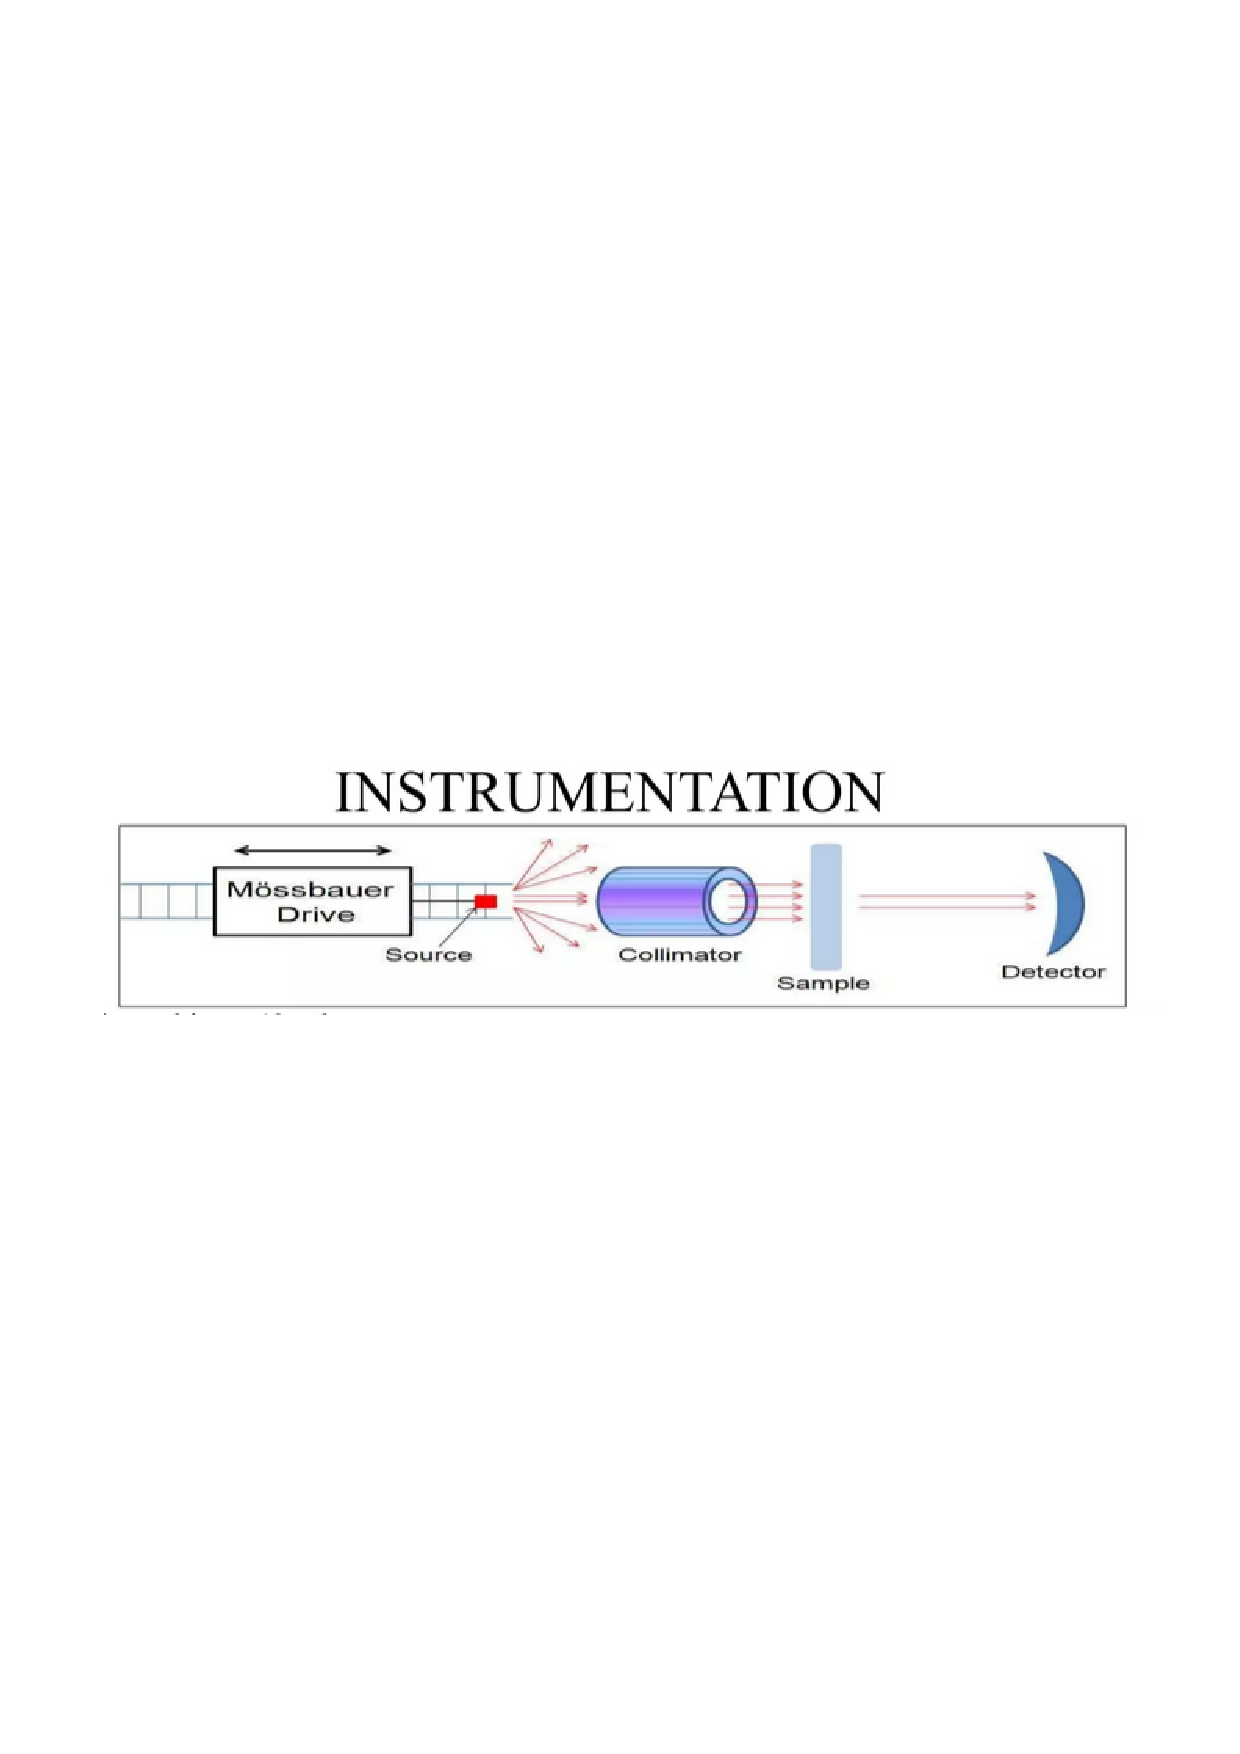
\includegraphics[width=0.8\linewidth, trim={1.5cm 11cm 1.5cm 11cm}, clip]{img/mossbauer_instrumentation.pdf}
    \caption{Experimentální uspořádání transmisní Mossbauerovy spektrometrie}
    \label{fig:2_6_mossbauer_zapojeni}
\end{figure}

%- můžu mít transmisní geometrii, odrazovou geometrii, můžu měřit konverzní elektrony
%- CEMS (Conversion Electrons Mossbauer Spectroscopy), TMS (Transmission Mossbauer Spectrometr), CXMS (Conversion X-ray Mossbauer Spectroscopy)
%- vzorek nesmí být ani moc tlustý, ani moc tenký - definuji efektivní tloušťku
%- jako detektory se využívají scintilárky, proporcionální detektory, polovodičové detektory nebo Si-PIN detektory
%- scintilační detektory NaI(Tl), YAP(Ce) 
%- proporcionální dteektory mají lepší rozlišení v porovnání se scintilákama
%

\subsubsection{Využití}

\begin{itemize}
    \item Mossbauerovské jádro mi funguje v mém materiálu jako sonda a říká mi informace o jeho okolí = lokální mikrostruktura
    \item Sledování hyperjmených interakcí Mossbauerovského jádra s jeho okolím = jedná se o interakce, které nějaký způsobem ovlivňují excitační stavy - Energetické stavy budou ovlivňovány svým okolím
    \item Mohu zkoumat vliv např. externího magnetického pole na posun či rozštěpení excitovaného či základního stavu (excitovaný/základní stav mají nějakou hladinu a buď může dojít vlivem externích jevů k jejich posuvu a nebo rozštěpení na více hladit)
    \item Informace o charakteru vazeb
    \item Informace o spinu
    \item Informace o oxidačním stavu
    \item Kvalitativní (identifikace sloučenin) i kvantitativní (poměrové zastoupení) např. fáze železa a jejich poměrové zastoupení i uspořádání. Interakce konkrétního nuklidu se svým okolím. 
    \item Využívá se především v materiálovém výzkumu a dále geologie, farmaceutický průmysl, biologie/medicín. Spíš ale prostě ten materiálový výzkum a je to.
\end{itemize}

\subsubsection{Hyperjemné interakce}

Jedná se o interakce, které nějaký způsobem ovlivňují excitační stavy, a to jak posunem nebo štěpením na více hladin. Bavíme se o:

\begin{itemize}
   \item elektrické monopólové interakci -- izomerický posun
   \item elektrická kvadrupólová -- kvadrupólové štěpení
   \item magnetická dipólová -- magnetické hyperjemné štěpení
\end{itemize}

\begin{figure}[H]
   \centering
   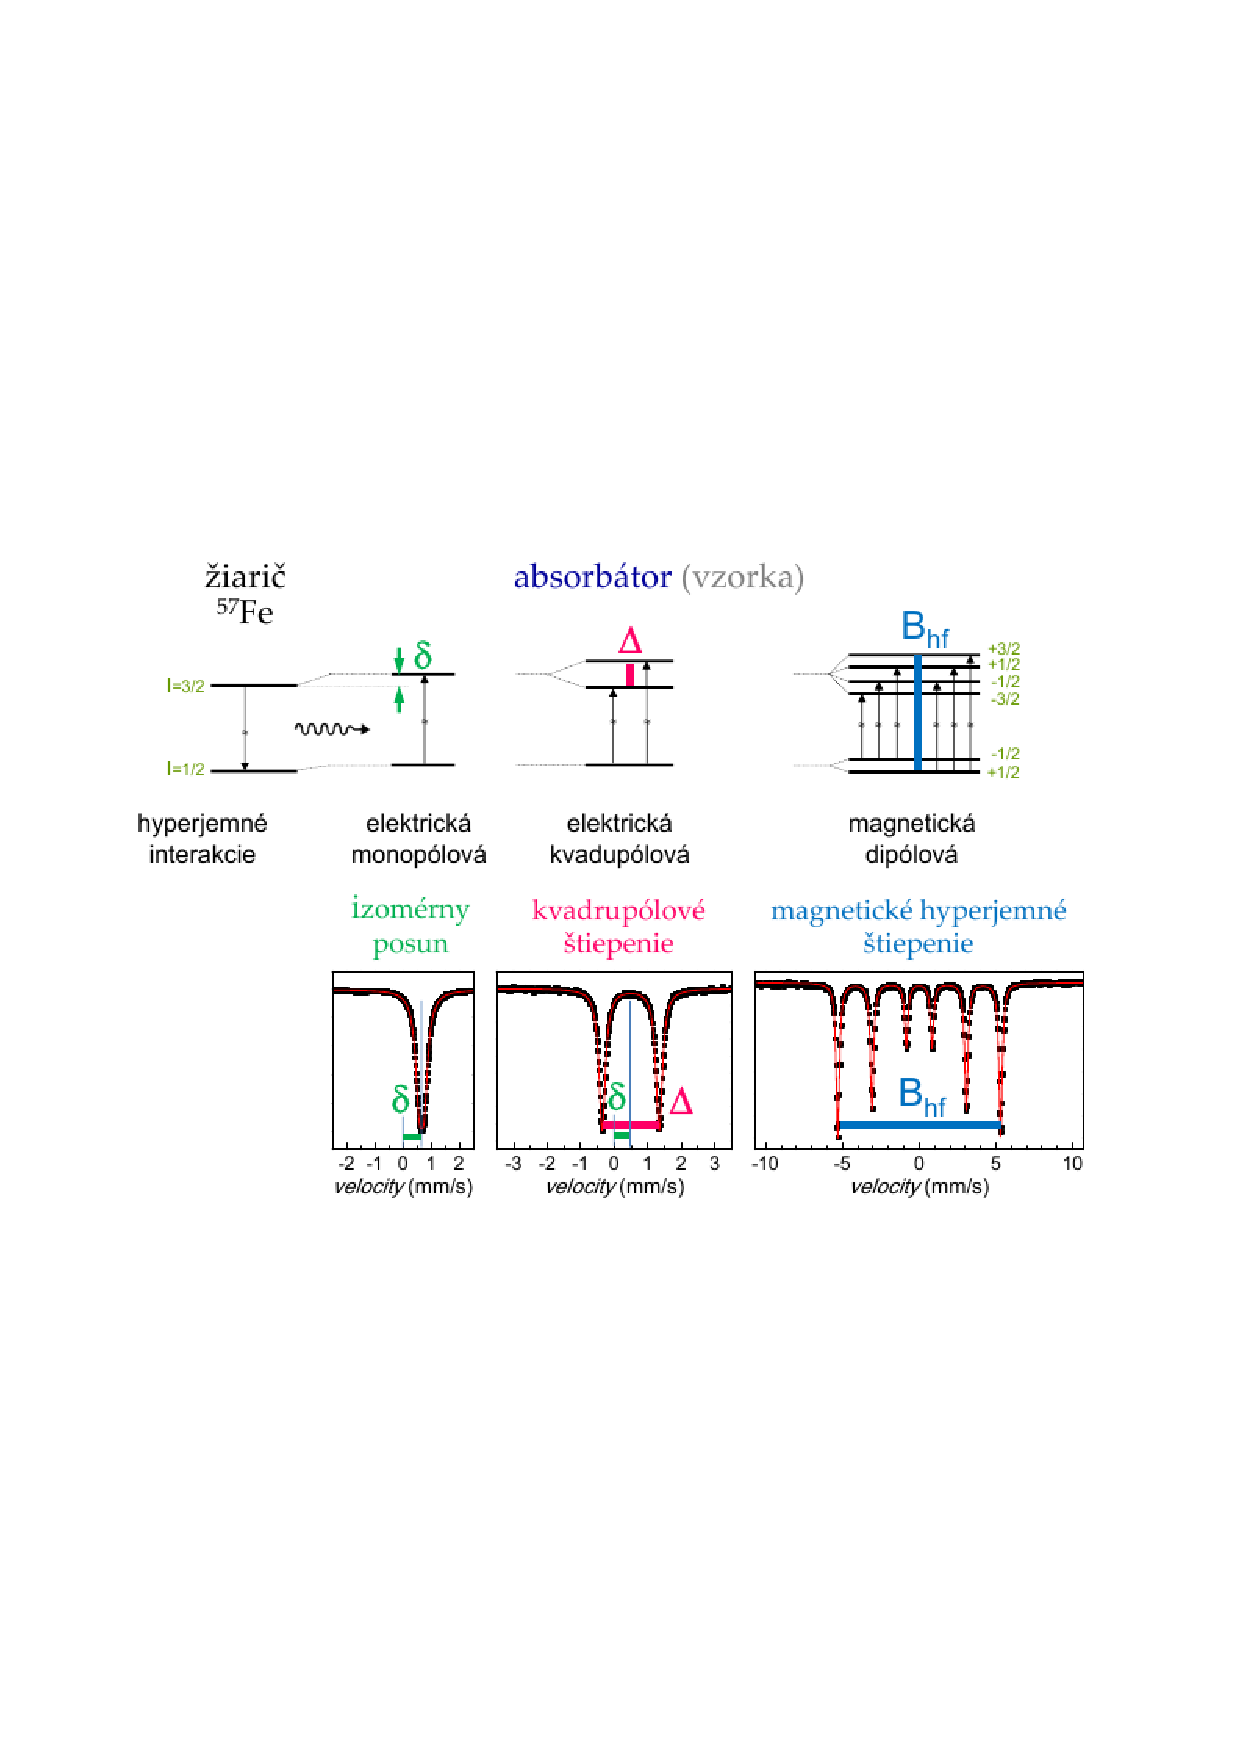
\includegraphics[width=0.8\linewidth, trim={2cm 10cm 2cm 10cm}, clip]{img/mossbauer_interactions.pdf}
   \caption{Hyperjemné interakce}
   \label{fig:6_2_mossbauer_hyperjemne_interakce}
\end{figure}

\textbf{Elektrická monopólová interakce:}

\begin{itemize}
\item interakce rozložení náboje jádra s hustotou elektronů v prostoru jádra 
\item izomerní posun $\delta = \dfrac{2\pi}{5} Ze^2 [R_e^2 - R_g^2] \cdot {\rho_a - \rho_s}$
\item pro excitovaný, resp. základní stav platí, že poloměr jádra se mění, stejně jako hustota
\item určuji s ohledem na referenční materiál (bcc-Fe)
\item udává informacee o charakteru vazeb, spinu, oxidačním čísle, elektronegativitě
\end{itemize}

\textbf{Elektrická kvadrupólová interakce:}

\begin{itemize}
\item interakce mezi jádrovým kvadrupólovým momentem a nehomogenitami elktrického pole
\item kvadrupólové štěpení: $\Delta = \dfrac{1}{2} eV_{zz} (1+\dfrac{1}{3}\eta^2)^{1/2}$ 
\item jaderná podmínka: elektrický kvadrupólový moment -- $eQ \neq$ 0 ($I$ > 1/2)
\item elektronová podmínka: gradient elektrického pole od elektronů $\neq$ 0 (příspěvek od mřížky a valenčních elektronů)
\item dává informaci o lókální symetrii, oxidačním stavu, charaktere vazeb, spinovém stavu

\end{itemize}
\begin{figure}[H]
   \centering
   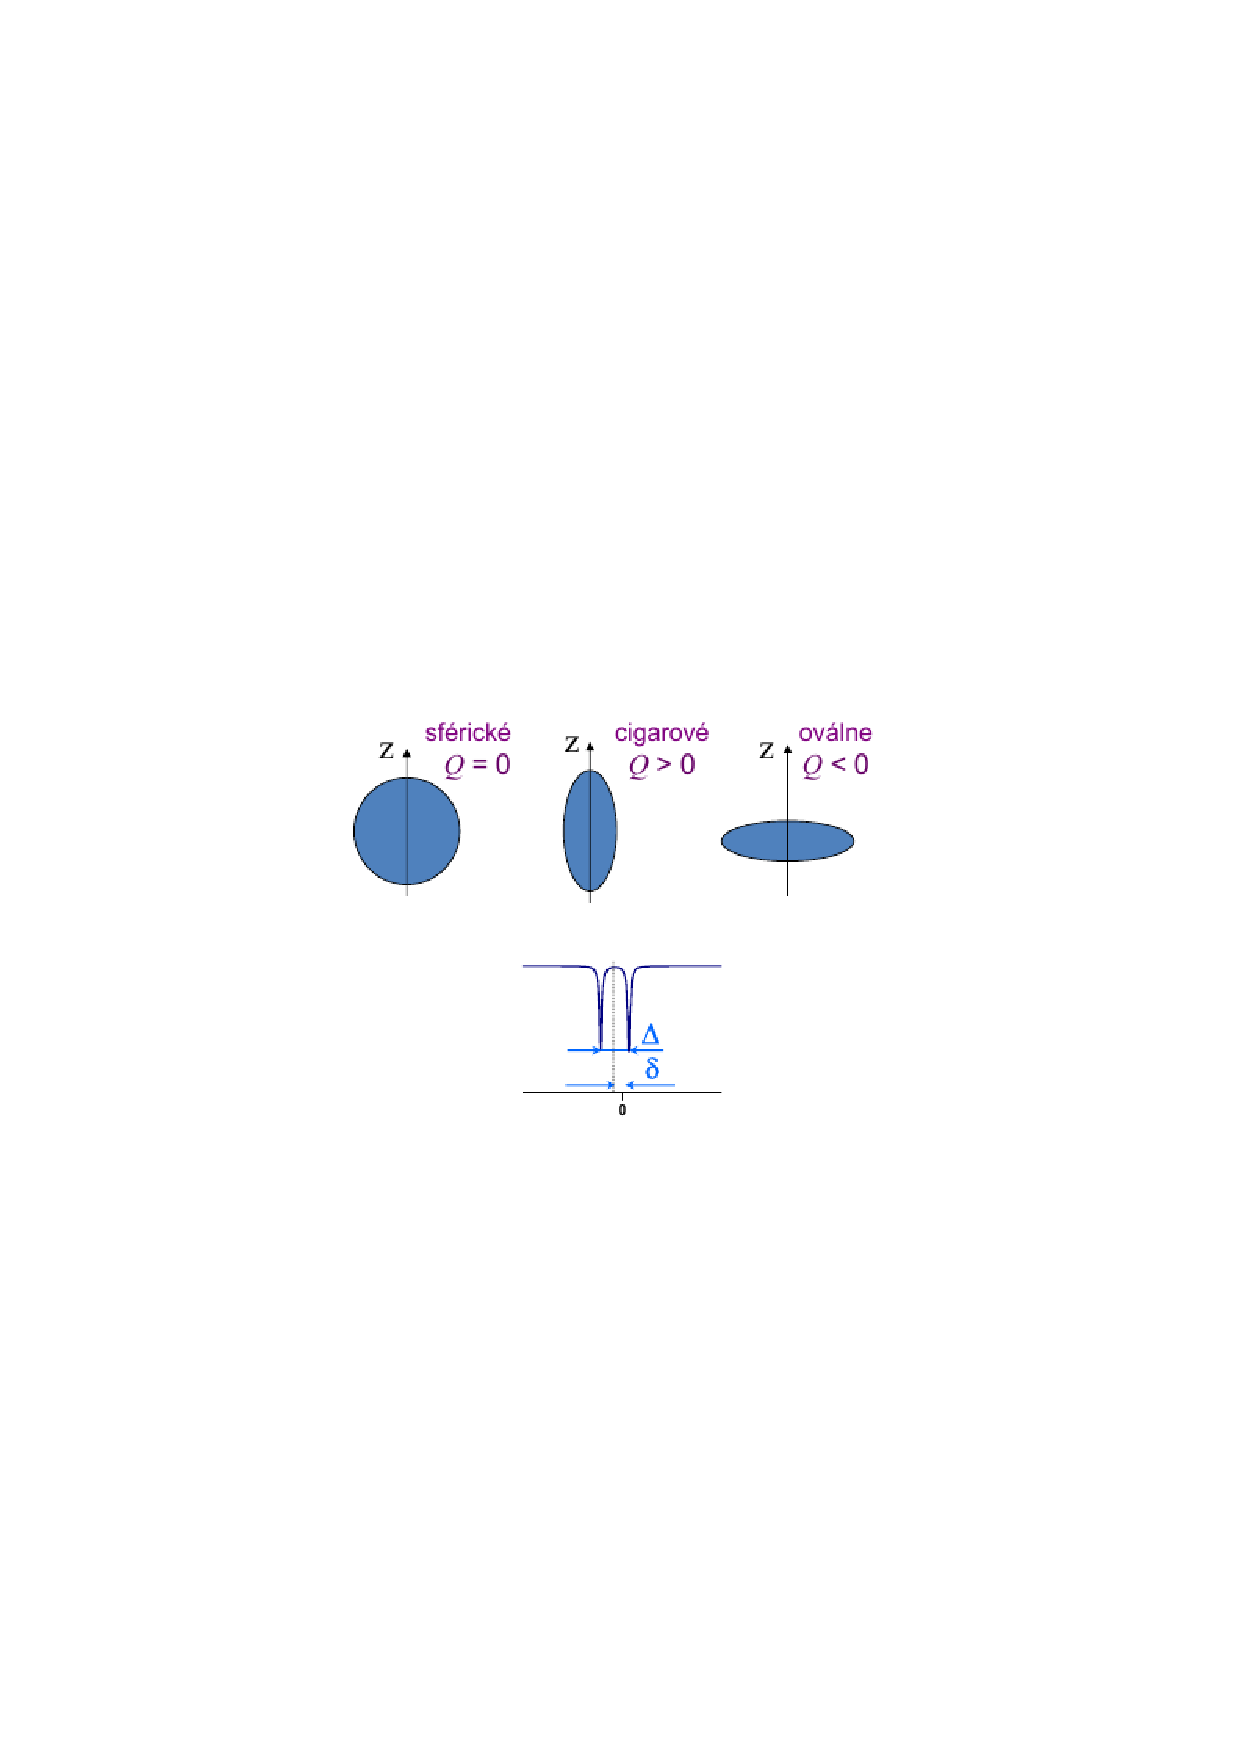
\includegraphics[width=0.5\linewidth, trim={4cm 11cm 4cm 11cm}, clip]{img/mossbauer_quadrupole.pdf}
   \caption{Elektrické kvadrupólové štěpení}
   \label{fig:6_2_mossbauer_electric_quadrupole}
\end{figure}

\textbf{Magnetická dipólová interakce:}

\begin{itemize}
   \item interakce magnetického momentu jádra s vnitřním nebo aplikovaným magnetickým polem
   \item $E_{m_1} = - \dfrac{\mu H m_1}{I} = - g_N \beta_N H m_1$
   \item magnetické štěpení hladin jádra (Zeemanův jev)
   \item jádrová podmínka: magnetický dipólový moment $\mu \neq 0$ (I > 0)
   \item elektronová podmínka: intenzita magnetického pole $H \neq 0$
   \item platí výběrová pravidla pro jádrový spin a magnetické kvantové číslo
\end{itemize}

\begin{figure}[H]
   \centering
   
\includegraphics[width=0.5\linewidth, trim={5cm 14cm 5cm 14cm}, clip]{img/mossbauer_magnetic_quadrupole.pdf}
   \caption{Magnetické kvadrupólové štěpení}
   \label{fig:6_2_mossbauer_magnetic_quadrupole}
\end{figure}

\subsubsection{Kalibrace}

\begin{itemize}
   \item zdroj záření: $^{57}$Co v matrici Rh, Pd, Cu, Cr
   \item kalibrací ryhlostní stupnice (převedu rychlost na energii)
   \item kalibrační absorbátory - bcc-Fe, $\alpha$-Fe$_2$O$_3$
   \item nastvaení nulové rychlosti
\end{itemize}

\subsubsection{APlikace Mossbauerovy spektrometrie}

\begin{itemize}
   \item strukturní informace, stechiometrie, substituce, nekrystalické systém
   \item identifikace fází
   \item Fe2+ a Fe3+
   \item energetické rozlišení 1 : 10$^{13}$
   \item teplotní a tlakové studie
\end{itemize}

\begin{figure}[H]
   \centering
   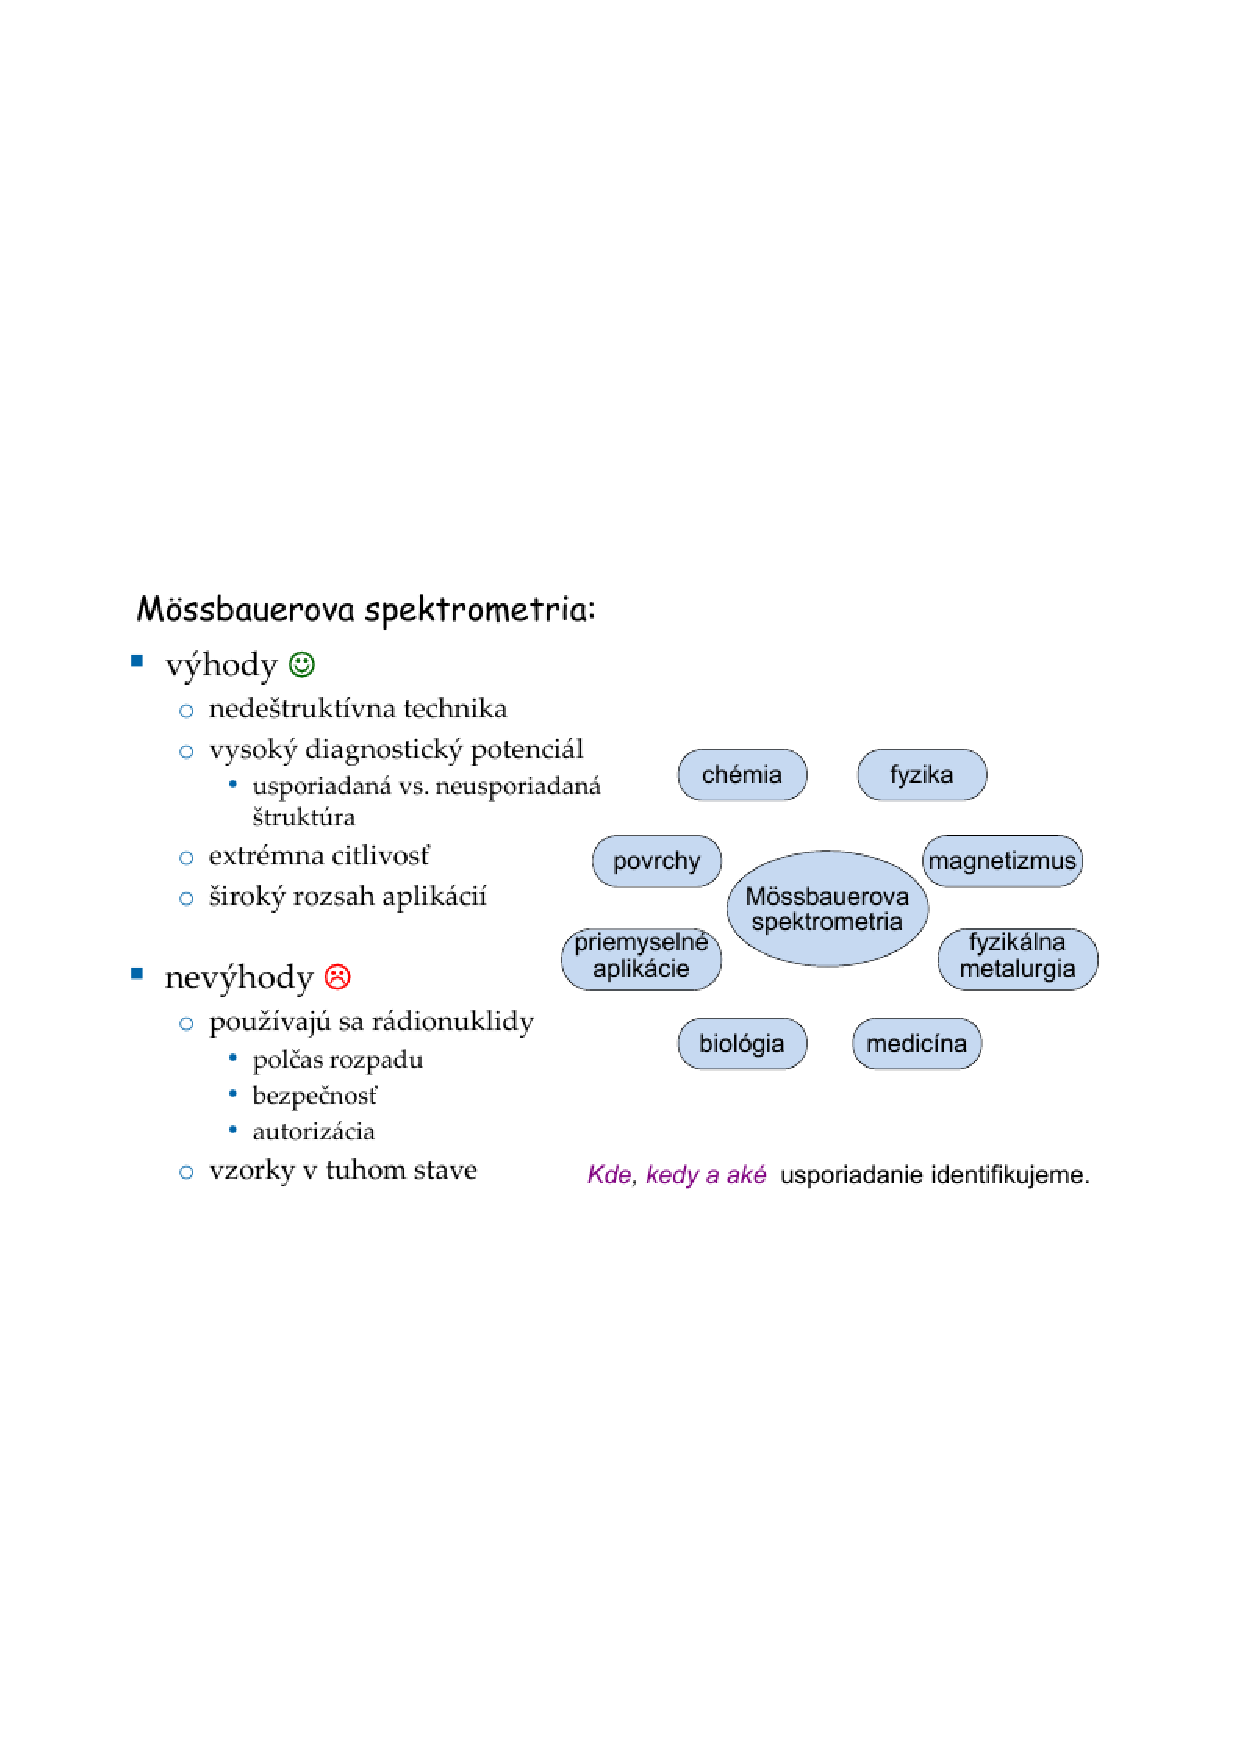
\includegraphics[width=0.5\linewidth, trim={2cm 10cm 2cm 10cm}, clip]{img/mossbauer_shrnuti.pdf}
\end{figure}

\subsection{Elektron-pozitronová anihilační spektroskopie}

Udává unikátní informace o defektech v pevných látkách (především vakance, dislokace, shluky vakancí, hranice zrn - principiálně se jedná o oblast se sníženou hustotou kladného náboje -- od jader :D $\rightarrow$ potenciálov jáma pro záchyt pozitronů).

Zdroje pozitronů:

\begin{itemize}
	\item beta+ radionuklidy: jádra bohatá na protony (p $\rightarrow$ n + $\beta$ + + $\nu$), Na-22, Cu-64, Co-58
	\item Produkce e--e+ párů z vysokoenergetických fotonů gama: impuzní zdroj e+
	\item Jaderné reakce: Cd-113(n, gama)Cd-114, Cu-63(n, gama)Cu-64, kontinuální zdroj s vysokou intenzitou
\end{itemize}

$\rightarrow$ Zdroje pro PET: C-11, N-13, O-15, \textbf{F-18}, Ga-68 - výroba: nejčastěji cyklotron

Princip anihilace: pozitronový zářič $\rightarrow$ interakce pozitronu s elektronem $\rightarrow$ vznik dvou fotonů o energii 511 keV (nejpravděpodobnější proce).

\begin{itemize}
    \item anihilace nenastává okamžitě - mezitím: vázaný stav - pozitronium (para a orto pozitronium - podle toho jestli stejný nebo opačný spin pozitronu a elektronu a také podle toho jinak dlouho trvají)
\end{itemize}

\subsubsection{Experimentální techniky}

\begin{itemize}
    \item Doba života pozitronů -- vyzářen pozitron a gama $\rightarrow$ měří se vyzáření pozitornu a gama
    \item Dopplerovo rozšíření -- koincidenční změření energie obou anihilačních fotonů $\rightarrow$ charakterizace chemického okolí defektů
    \item Úhlové korelace
\end{itemize}

\begin{figure}[H]
    \centering
    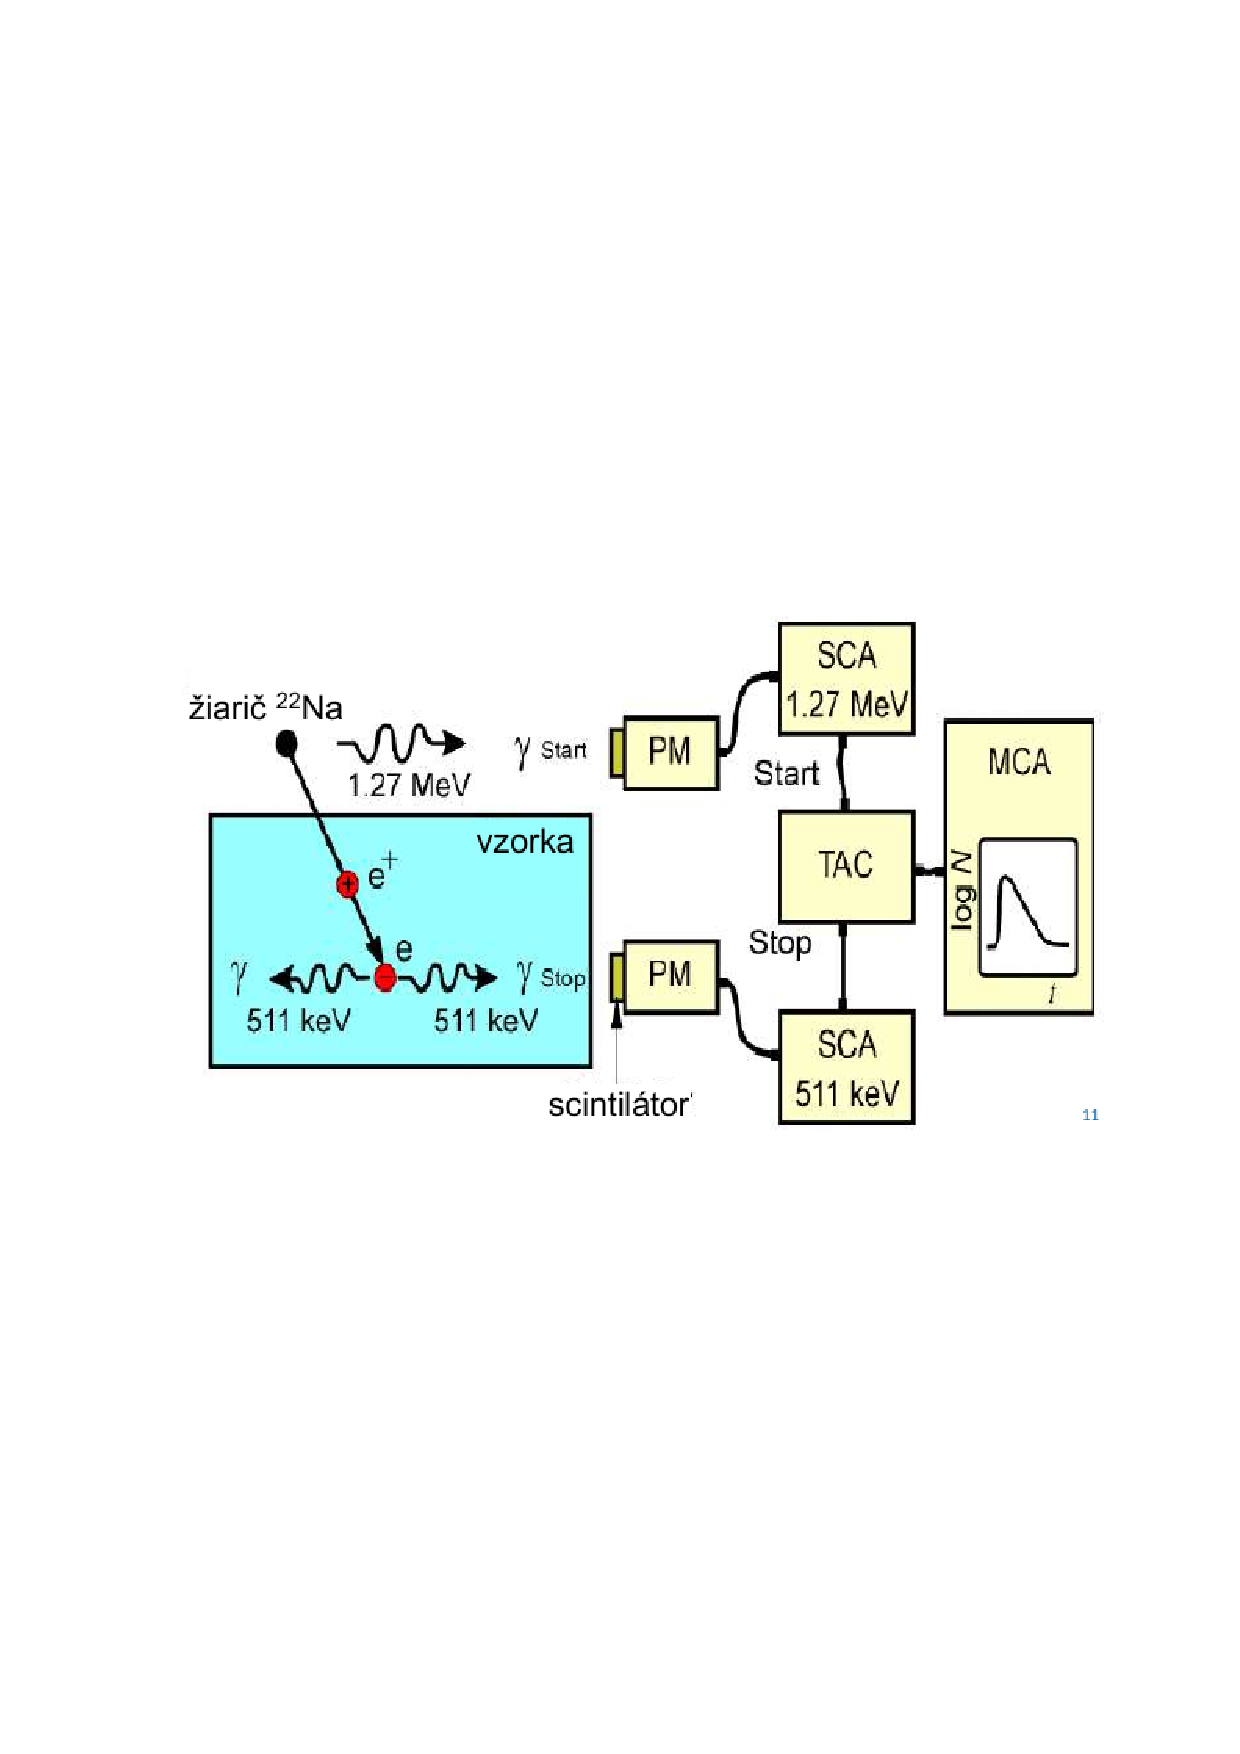
\includegraphics[width=0.8\linewidth, trim={2cm 10cm 2cm 10cm}, clip]{img/pas_doba_zivota.pdf}
    \caption{Metoda doby života pozitronů.}
    \label{fig:6_2_pas_doba_zivota}
\end{figure}

\begin{figure}[H]
    \centering
    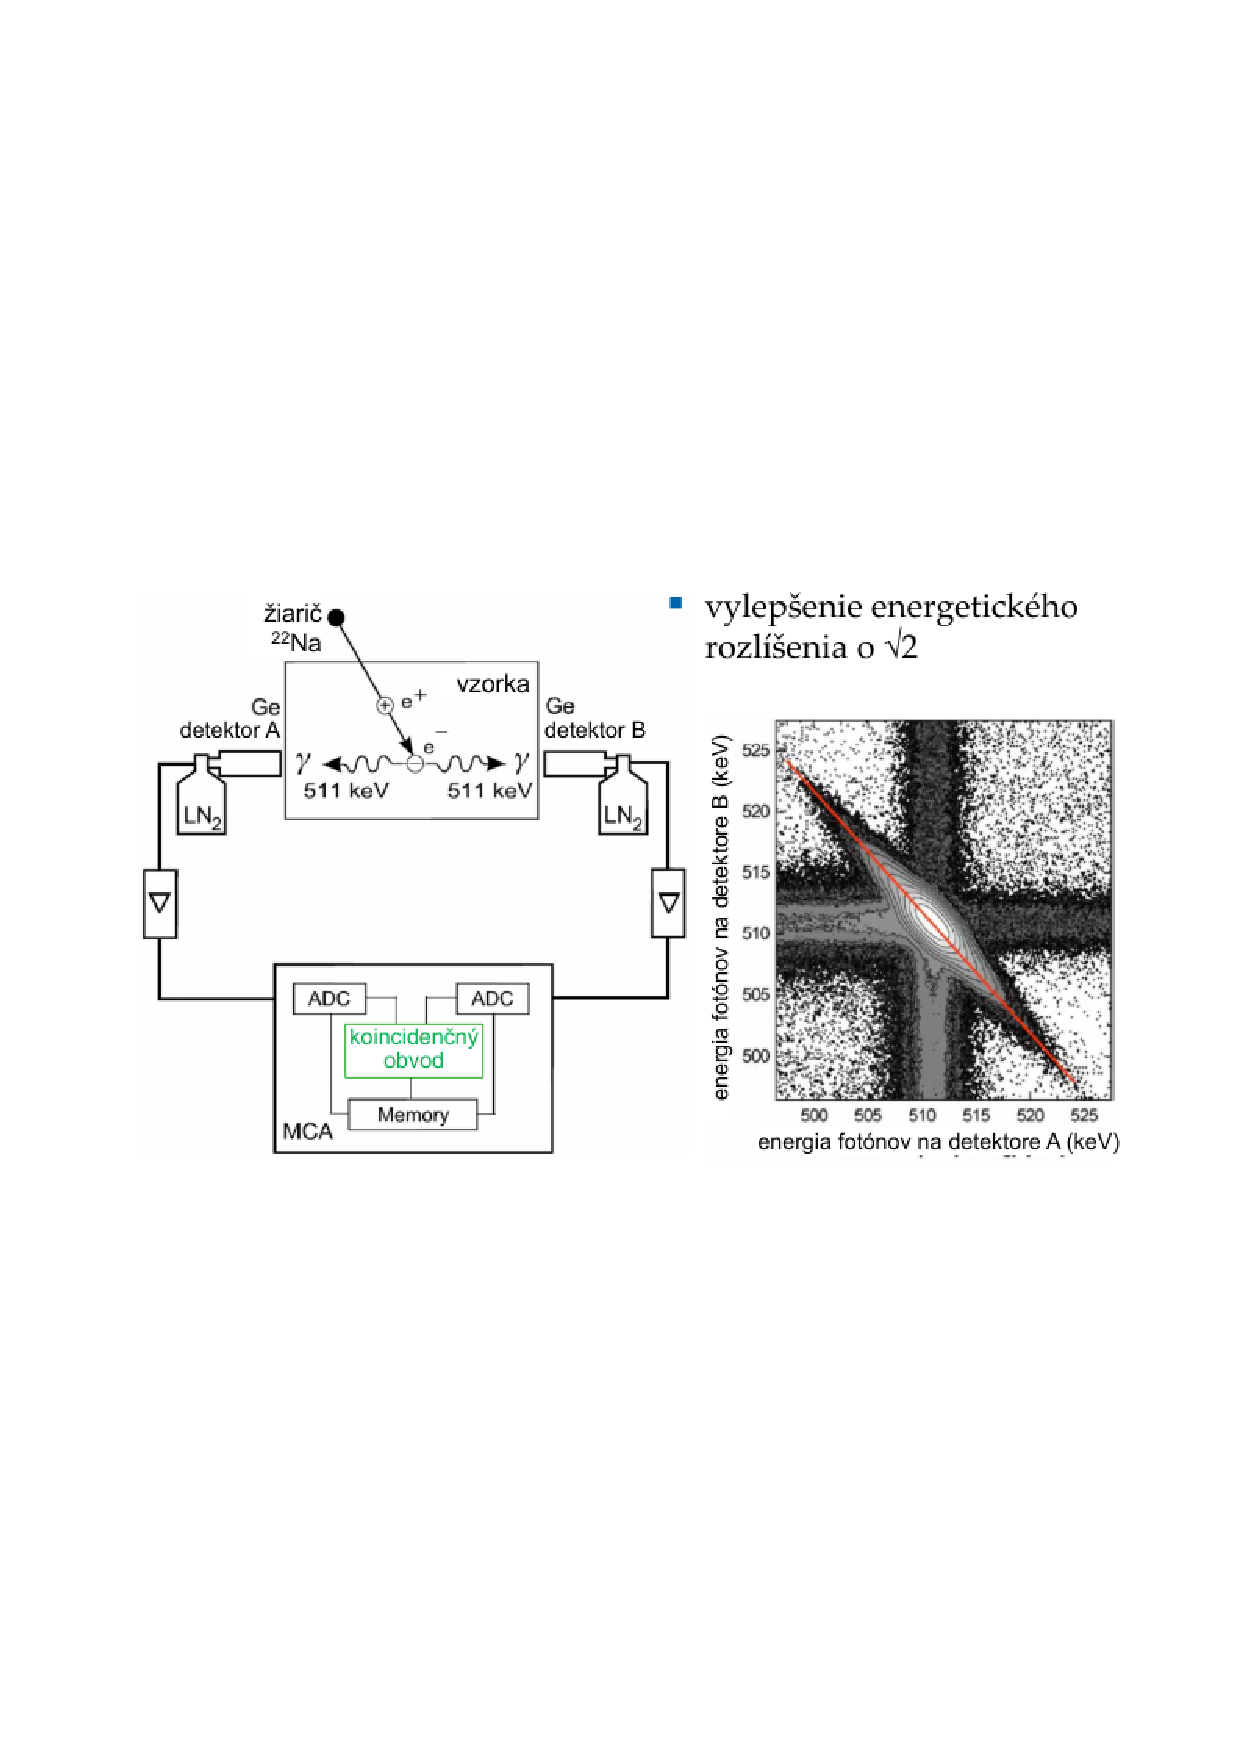
\includegraphics[width=0.8\linewidth, trim={2cm 10cm 2cm 10cm}, clip]{img/dopplerovo_koincidencni_zapojeni.pdf}
    \caption{Metoda Dopplerova rozšíření- koincidenční zapojení}
    \label{fig:6_2_pas_dopplerovo_rozsireni}
\end{figure}

\subsection{Neutronová aktivační analýza}

\begin{itemize}
    \item Je založena na aktivaci chemických prvků přítomných v analyzovaném vzorku. 
    \item Jedná se o jednu z nejvíce citlivých metod chemické analýzy
    \item Obvykle je aplikována s využitím měření následného rozpadu aktivovaných prvků (měření gama)
    \item Existuje i metoda s měřením okamžitého záření a ta je využívána pokud produkt reakce má velmi krátký poločas rozpadu a nebo vzniká stabilní produkt.
    \item Pro NAA se dají vyuźít neutrony všech energií, avšak nejčastěji se využívají tepelné, a to kvůli větší dostupnosti neutronů při této energii a také kvůli energetické závislosti účinných průřezů, které mají v této oblasti vysoké hodnoty.
    \item Množství aktivovaných RA atomů daného prvků ve vzorku je přímo úměrné množství těchto atomů a proto se dá využít i pro kvantitativní analýzu.
    \item Indukovaná aktivita závisí na době ozařování a poločasu rozpadu, přičemž okolo $10x T_{1/2}$ dosahuje akivita saturované hodnoty.
    \item Po aktivaci jader v analyzovaném vzorku následuje měření radioaktivity vzorku a identifikace RN na základě energie a intenzity emitovaného gama záření a s ohledem na poločas rozpadu.
    \item Množství studovaného prvku lze získat z naměřené aktivity s tím, že je nutno brát v potaz:
    \begin{itemize}
        \item Hustotu toku neutronů (resp. energetické spektrum)
        \item Energetickou závislost účinných průřezů
        \item Dobu ozařování
        \item Poločas rozpadu
        \item Detekční účinnost trasy (geometrie, stínění, mrtvá doba atd.)
        \item Dobu měření
        \item Dobu chladnutí (přesun po ozařování k detektoru)
    \end{itemize}
\end{itemize}
 
\textbf{Rozdělení NAA}
\begin{itemize}
    \item Absolutní
        \begin{itemize}
            \item Z přímého měření aktivity umožňuje stanovit množství zkoumaného izotopu, avšak vyžaduje k tomu přesnou znalost neutronového spektra, účinných průřezů s ohledem na energetický rozsah neutronového pole.
            \item Málo kdy využívaný přístup protože přesná znalost neutronového spektra není v praxi obvykle k dispozici
        \end{itemize}
    \item Porovnávací:
        \begin{itemize}
            \item Srovnávání aktivity RN ve zkoumaném vzorku s jeho aktivitou v podobě standardu/etalonu o známé hmotnosti a složení, který byl ozářen za stejných podmínek jako zkoumaný vzorek
            \item Při srovnávací metodě se nevyužívají hodnoty účinných průřezů ani neutronový tok a v případě stejné geometrie při detekci/měření tak ani absolutní detekční účinnost (pro oba měřené je to stejné, tak to není vyžadováno)
            \item Vysoká přesnost, avšak časově náročné pokud vzorek obsahuje vícero prvků, protože pro každý je nutné mít etalon zvlášť.
        \end{itemize}
    \item $k_0$ metoda
        \begin{itemize}
            \item využívá $k_0$ faktory, které se stanovují na základě jaderných dat v kombinaci s experimentálním stanovením.
            \item nezávisí na neutronovém toku a charakteristikách detektoru
        \end{itemize}
    \item Instrumentální NAA -- toto známe a děláme na KJR.
        \begin{itemize}
            \item Nedestruktivní metoda pro stanovení vícero prvků v rámci jednoho měření
            \item Nežádoucím efektem je vzájemné ovlivňování prvků = Vznik jednoho RN reakcemi na dvou různých prvcích (26Mg(n;$\gamma$)27Mg a 27Al(n;p)27Mg) = Tento problém je ovšem řešitelný v případě, kdy jeden z prvků produkuje i další radioaktivní nuklidy a dále také pokud je rozdíl v energetické závislosti účinných průřezů na energii neutronů, tak se dá použít vhodný filtr jako např Cd.
            \item V praxi se měří tak, že se vzorek ozáří v reaktoru na saturovanou hodnotu, pak se nechá vychladnout (snížení aktivity) pokud je moc naaktivovaný a pak se odnese do gama spektrometru a měří se gama záření z rozpadu RN. Z naměřeného spektra se poté stanovuje kvantita a kvalita složení materiálu.
        \end{itemize}
\end{itemize}

\subsubsection{Nastavení experimentálních parametrů}
\begin{itemize}

            \item V rámci tohoto měření, tak je vhodné mít odladěnou dobu ozařování (ať to není zbytečně moc a aktivita dlouhodobě žijících RN není moc vysoká)
            \item dobu vymření (chceme minimalizovat aktivitu všech RN kromě toho, který chceme měřit)
            \item Doba měření (měla by být kratší než nějaký významnější pokles aktivity vzorku - pak mi do toho začne hrát roli pozadí a Rn, K a U)
            \item při ozařování dochází ke vzniku vícero aktivačních produktů z jednoho prvku (pro ověření lze měřit dlouho a zaměřit se na ověření přes poločas rozpadu). Popřípadě aktivační produkty obvykkle emitují $\gamma$ fotony o vícero energiích, čímž je možné taky jednoznačně stanovit.
            \item Měřící geometrie (mrtvá doba)
            \item Velikost vzorku: zbytečně velký vzorek představuje riziko samostínění, samoabsorpce gama záření či zbytečně velkou aktivitu nebo problematické manipulace (to platí i pro zbytečně malý vzorek).
            \item Tok primárních částic přímo ovlivňuje úroveň produkované aktivity.
            \item Ve výsledném výpočtu reakční rychlosti, resp. obecně měření je nutné zohlednit několik faktorů = plocha pod píkem při měření, počet částic v látce na počátku, oprava na čistou dobu měření, doba ozařování, rozpad při vymírání, rozpad při měření, Radiační výtěžek (oprava na intenzitu gama přechodu), oprava na efektivitu detektoru pro danou geometrii (detekční účinnost). Korekce na nerovnoměrné ozařování, korekce na samoabsorpci.
        \end{itemize}

\textbf{Využití a aplikace NAA:}
\begin{itemize}
    \item Monitoring životního prostředí
    \item Zajištění jakosti v průmyslu
    \item Hygienické studie
    \item Certifikace referenčních materiálů
    \item Stopové prvky
    \item Kvalita půdy
    \item Analýza uhlí
\end{itemize}
\section[Jaderně-fyzikální metody v nukleární medicíně]{Jaderně-fyzikální metody v nukleární medicíně: gama kamera, CT, PET}


\section[Využití synchrotronového záření v materiálovém výzkumu]{Využití synchrotronového záření v materiálovém výzkumu: získávání synchrotronového záření a jeho vlastnosti, příklady experimentálních technik}


\section[Jednotky a veličiny v dozimetrii]{Jednotky a veličiny v dozimetrii, základy legální metrologie, etalony a stanovená měřidla}

Metrologie je věda zabývající se měřením . Mezi základní cíle a úkoly patří:

\begin{itemize}
    \item definice jednotek a jejich realizace pomocí vědeckých metod,
    \item vývoj a udržování etalonů nejvyšší úrovně,
    \item zajištění fungování měřidel ve výrobní sféře,
    \item zajistit správnost měření v úředních nebo obchodních sférách,
\end{itemize}

\subsection{Základy legální metrologie}

Hlavním je zákon č. 505/1990 Sb. o metrologii $\rightarrow$ upravuje práva a povinnosti subjektů a státních orgánů správy pro účely zajištění správnosti a jednotnosti měřidel a měření.
Dále jsou důležité prováděcí vyhlášky k samotnému zákonu, a to sice:

\begin{itemize}
    \item Vyhláška MPO č. 262/2000 Sb., kterou je zajišťována jednotnost a správnost měřidel a měření.
    \item Vyhláška MPO č. 345/2002 Sb., kterou se stanoví měřidla k povinnému ověřování a měřidla podléhající schvalování.
    \item Vyhláška MPO č. 264/2000 Sb., o základních měřících jednotkách a ostatních jednotkách a o jejich označování.
\end{itemize}

Klasifikace měřidel:

\begin{itemize}
    \item \textbf{Etalony} (primární, sekundární, mezinárodní, státní) = objekt či něco jiného, jež obecně slouží k uchování a realizaci dané jednotky (etalon hmotnosti, kde jednotka je kg, tak je snad krystal křemíku, protože umíme přesně určit počet atomů v mřížce).
    \item \textbf{Stanovená měřidla} = Jedná se o měřidla, která MPO (ministerstvo průmyslu a obchodu) vyhláškou stanoví k povinnému ověřování s ohledem na jejich význam (obchod, daně, sankce, tarify, poplatky, medicína, ochrana ŽP, BOZP).
    \item \textbf{Pracovní měřidla} = jedná se o měřidla jež nejsou etalonem ani stanoveným měřidlem.
    \item \textbf{Certifikované a ostatní referenční materiály} = Jedná se o materiály přesně stanoveného a známého chemického složení, které slouží pro ověřování nebo ke kalibraci (často to bývají etalony)
\end{itemize}

Schvalování typů měřidel je proces, při kterém jsou ověřeny metrologické a technické vlastnosti stanovených měřidel, jež vycházejí z technických norem. Zkoušky pro schválení typu stanoveného měřidla obsahuji funkční zkoušky, zkoušky odolnosti proti rušivým vlivům vnějšího prostředí a zkoušky elektromagnetické kompatibility. Výsledkem je certifikát a přidělení značky schválení typu.

Pod pojmem \textbf{návaznost} rozumíme: (definice je na hovno) V zásadě se jedná o to, že vemu např. 8 vah z celého světa, nastavím je pomocí kvalitního etalonu na to, že toto je 1 kg a potom, když něco naměřím já, tak i Karlíkovi z horní dolní můžu věřit, že to má jak já, protože to má nastavený v návaznosti na ten samý etalon a tudíž i v návaznosti na mne.

\textbf{Ověřování} je proces, resp. potvrzení, že měřidlo má požadované metrologické vlastnosti.

\textbf{Kalibrace} je proces, kdy je periodicky upravováno a kontrolováno, že měřidlo měří to co má a případná kalibrace probíhá pomocí certifikovaných a ostatních referenčních materiálu, kterými jsou nejčastěji etalony.

\subsubsection{Organizace}

\textbf{ÚNMZ = Ústav pro technickou normalizaci, metrologii a státní zkušebnictví}

\begin{itemize}
    \item Zastupování ČR ve věci mezinárodních věcí s ohledem na metrologii.
    \item Dohled na činnosti ČMI.
    \item Kontrola dodržování zákona o metrologii.
    \item Schválení a vyhlášení státních etalonů.
    \item Poskytování metrologických expertíz.
\end{itemize}

\textbf{ČMI}

\begin{itemize}
    \item Uchovávání a rozvoj státních etalonů.
    \item Schvalování typů a ověřování stanovených měřidel.
    \item Certifikace referenčních materiálů.
    \item Kalibrační služby.
\end{itemize}

\subsubsection{Veličiny a jednotky}

Existují různé soustavy jednotek, kde nejvíce je rozšířené SI, dále existuje imperiální, americká apod... Stačí znát SI.

V obecnosti jsou základní jednotky SI popsáné v Zákoně č. 505/1999 Sb. o metrologii. Obsaženy jsou dále odvozené jednotky, násobky, díky a jiné povolené jednotky.

Základní jednotky a veličiny SI jsou:

\begin{itemize}
    \item Čas -- s,
    \item Proud -- A,
    \item Svítivost -- cd,
    \item Látkové množství -- mol,
    \item Teplota -- K,
    \item Hmotnost -- kg,
    \item Délka -- m.
\end{itemize}

Odvozené jednotky vyjadřované jednotkami základními jsou např. hustota, objem, plocha, rychlost, ...

Odvozené jednotky se zvláštním označením i názvem jsou např. náboj, síla, aktivita, absorbovaná dávka, ...

Odvozené jednotky vyjádřené jednotkami základními spolu s jednotkami se zvláštním názvem a označením jsou např. Expozice, PDE, dávkový příkon, dávkový ekvivalent, ...

\textbf{Vlastnosti a výhody SI:}

\begin{itemize}
    \item Systematická a mezinárodně uznávaná soustava veličin a jednotek.
    \item Pro každou veličinu zavedena pouze jedna jednotka.
    \item Odvozené jednotky tvořeny součiny mocnin základních jednotek.
    \item Násobky a díly jednotek vyjádřeny předponami.
\end{itemize}

\textbf{Další mimosoustavné jednotky:} Jsou použitelné spolu s SI v rámci specifikovaných oborů a nebo výjimečně a tehdy, jeli definován vztah k SI jednotkám: uzel, dioptrie, angstrom, barn, atm, curie, calorie.

\textbf{Veličiny ve vztahu k atomové a jaderné fyzice:} Aktivita, přeměnová konstanta, poločas rozpadu, barn, hustota toku, fluence, absorbovaná dávka, kerma, expozice, dávkový ekvivalent, efektivní dávka, PDE, ...

\subsection{Jednotky a veličiny v dozimetrii}

\textbf{Expozice:}

Definována pro popis ionizujících účinků fotonů ve vzduchu: $[X] = C \cdot \text{kg}^{-1}$.

Expozice je definována jako podíl celkového náboje d$Q$ iontů jednoho znaménka, jež vznikly při úplném zabrzdění všech elektronů a pozitronů uvolněných fotony v malém objemu vzduchu, a hmotnosti tohoto objemu vzduchu d$m$.

\begin{equation}
    X = \frac{\text{d}Q}{\text{d}m}
\end{equation}

\begin{figure}[H]
    \centering
    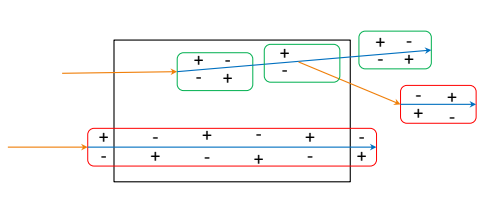
\includegraphics[width=0.5\linewidth]{img/expozice.png}
    \caption{expozice}
\end{figure}

\textbf{Absorbovaná dávka}

Vyjadřuje střední energii předanou IZ dané látce o jednotkové hmotnosti: $[D] = \text{Gy}$.

\begin{equation}
    D = \frac{\text{d}\overline{\varepsilon}}{\text{d}m}
\end{equation}

\textbf{Kerma}

Popisuje působení nepřímo ionizujícího záření z hlediska energetických ztrát primárních částic: $[K] = \text{Gy}$.

\begin{equation}
    K = \frac{\text{d}E_k}{\text{d}m}
\end{equation}

\textbf{Dávkový ekvivalent, resp. ekvivalentní dávka}

Jedná se o veličinu jž využívá tzv. faktoru kvality $Q$, kterým je přenásobena absrobovaná dávka a tento faktor kvality pak popisuje vliv daného IZ na tkáň (bez rozdělování o jakou tkáň se jedná): $[H] = \text{Sv}$.

$Q = 1$ pro elektrony, gama a RTG, dále je $Q = 10$ pro protony, neutrony a $Q = 20$ pro nabité ionty, alfa částice, štěpné produkty.

\begin{equation}
    H = Q \cdot D
\end{equation}    


\textbf{Efektivní dávka}

Jedná se o Dávkový ekvivalent násobený dalším faktorem kvality, a to tentokrát tkáňovým faktorem, který zohledňuje ještě dále, jaká část těla schytala to záření, protože každá část těla je jinak náchylná/odolná. To v praxi znamená, že kostní dřeň je snad nejvíce náchylná, zatímco játra nebo oko, dlaň (kůže) není tolik: $[D] = \text{Sv}$.

\begin{equation}
    D \cdot w_r = H, E = \sum_T w_T \cdot H_T
\end{equation}


\section[Využití detektorů v metrologii aktivity]{Využití proporcionálních detektorů a kapalných scintilátorů v metrologii aktivity radionuklidů}

Metrologie radioaktivity radionuklidů je dělena do dvou základních skupin:

\begin{itemize}
    \item Absolutní = Využívá přímé detekce veličiny (Koincidenční metoda, elektrostatická metoda, kalorimetrická metoda, absolutní počítání částic).
    \item Relativní = Vztah mezi veličinou indikovanou a veličinou měřenou (spektrometrie gama, ionizační komora).
\end{itemize}

\subsection{Využití proporcionálních detektorů}

Jedná se o primární metodu měření = vychází z definice veličiny.

Proporcionální detektor je často válcové geometrie a skládá se z anody (tenký drátek z W, Mo, Cu, ocel, Au pokrytí) a katody (tělo detektoru). Díky velkému rozdílu ve velikosti elektrod je mezi nimi velký rozdíl napětí, a to vytváří velmi intenzivní elektrické pole. Pracovním plynem uvnitř detektoru je často Ar, Kr, Xe + zhášecí plyn, což je například Metan nebo propanbutan.

Výstupní impuls na detektoru je úměrný deponované energii. Typická náplň je plyn P-10 (90\% Ar a 10\% CH$_4$).

Důležité je, aby anodový drátek měl konst. průměr a tloušťku. Výhodou proporcionálního detektoru je, že téměř nemá mrtvou dobu a je tedy hodně dobře schopen detekovat dva signály "naráz".

Je provozován v oblasti proporcionality VA charakteristiky plynového detektoru, kdy měřená četnost téměř nezávisí na napětí (pracovní napětí detektoru je zvoleno v této oblasti). Provoz v této oblasti umožňuje rozvoj townsendovy laviny, jež představuje plynové zesílení.

Plynová naplň v detektoru je přítomna za účelem zesílení vstupního signálu = plynové zesílení. Proto je proporcionální počítač vhodný pro detekci záření malých energií, které je pak třeba zesílit právě přítomným plynem (ionizace plynu k zesílení vstupního signálu, a to řádové E2 až E3).

Proporcionální počítač se používá k měření $\alpha$ a $\beta$ záření.

Proporcionální počítače lze využít jako prosté detektory čítání, ale také částečně pro spektrometrii/spektroskopii neboť výstupní signál je úměrný vstupnímu, resp. deponované energii (s uvážením zesílení od plynu).

\textbf{Druhy proporcionálních počítačů:}

\begin{itemize}

    \item Průtokový: 

        \begin{itemize}
            \item Pracovní plyn protéká detektorem o atmosférickém tlaku a díky tomu je snadná výměna vzorků.
            \item Měření $\alpha$ a $\beta$ záření, zejména pak $\beta$.
            \item Lze udělat i 4$\pi$ variantu.
            \item Vhodný pro měření nízkoenergetické $\beta$ a plynných radioaktivních sloučenin i neutronů (pro neutrony je potřeba konverzní materiál).
        \end{itemize}
    
    \item Tlakový: 

        \begin{itemize}
            \item Plynová náplň má vyšší hmotnostní číslo a plyn je natlakován do cca 1,5 MPa.
            \item Vyšší tlak umožňuje dosáhnout vyšší účinnosti detekce záření (Tím, že je to natlakované, tak se tam vejde více plynu a tím se mi zvyšuje pravděpodobnost interakce záření s plynem).
        \end{itemize}

\end{itemize}


\textbf{Korekce:}

Zejména pro interní proporcionální poćítač, kdy je měřený vzorek uvnitř.

\begin{itemize}
    \item Koncový efekt = Na okrajích elektrod je elektrické pole deformované. Lze kompenzovat využitím dvou počítačů různé délky a rozdíl odezvy odpovídá četnosti naměřené ideálním detektorem o délce rozdílu jejich délek.
    \item Stěnový efekt = částice emitovaná v blízkosti stěn nestačí dostatečně ionizovat (oprava na základě měření s několika počítači stejné délky různých poloměrů, vliv klesá s rostoucím tlakem plynové náplně)
\end{itemize}

\subsection{Využití kapalných scintilátorů}

Jedná se o scintilační detektor, kde scintilační látka je tekutá/roztok. Jedná se o roztoky scintilačních látek v organických rozpouštědlech + měřený vzorek, který je v tomto taktéž rozpuštěn (podle druhu měřeného vzorku se používají rozpouštědla jako je toulen, xylen, ethalon).

Kapalné scintilátory se používají pro detekci IZ ($\alpha$ a $\beta$) o vyšších energiích (minimální detekovatelná energie je 3-10 keV). Využívají se pro tzv. metodu TDCR (triple to double coincidence ratio).

Detekční účinnost je dána účinnosti fotokatody daného fotonásobiče (kvalita fotonásobiče).

\subsubsection{TDCR}

Jedná se o koincidenční zapojení tří fotonásobičů, jež funguje na principu poměru trojných a dvojných koincidencí. Tato metoda slouží ke stanovení počítací účinnosti, a to experimentálně bez potřeby kalibračního standardu.

počítací účinnost ($\varepsilon_D$), neboli parametr TDCR (v zásadě detekční účinnost) se určuje na základě srovnání experimentu a modelu $\rightarrow$ v praxi je měřeno TDCR pro různé účinnosti detekce, které mohu měnit defokusací PMT, optickými filtry atd. Tím získávám závislost naměřené aktivity na TDCR (aktivita by měla být nezávislá na TDCR - kritérium správnosti) a dále závislost detekční účinnosti na TDCR (tu detekční účinnost si měním). Ve výsledku srovnáním experimentu a modelu získám účinnost $\varepsilon_D$:

$$ \left( \frac{\varepsilon_T}{\varepsilon_D} \right)_\text{výpočet} = \left( \frac{N_T}{N_D} \right)_\text{měření}. $$

Výsledný počet řešení TDCR parametru se odvíjí od druhu radionuklidu a složitosti jeho kaskády rozpadu.

Výsledná aktivita je získána jako: 

$$ A = \frac{N_D}{\varepsilon_D}. $$

\begin{figure}[ht!]
    \centering
    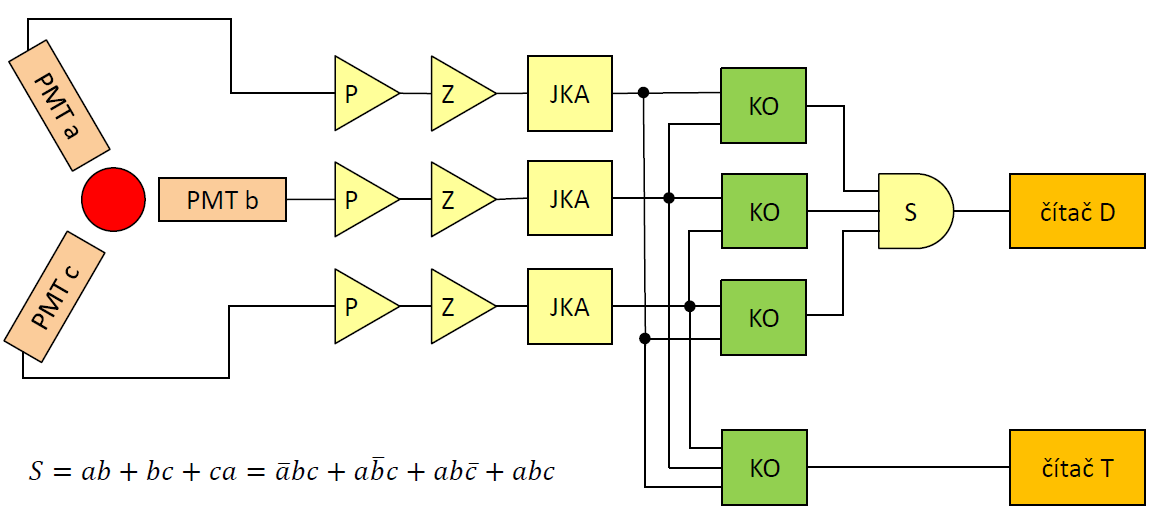
\includegraphics[width=1\linewidth]{img/tdcr.png}
    \caption{TDCR}
\end{figure}

\section[Koincidenční metoda \& spektrometrie gama]{Koincidenční metoda stanovení aktivity a spektrometrie záření gama jako sekundární metoda měření aktivity}


\section[Metrologie neutronů \& manganová lázeň]{Metrologie neutronů a metoda manganové lázně včetně zpracování výsledků měření a zdrojů chyb a nejistot}

Z hlediska metrologie neutronů je dobré zmínit nejprve veličiny jako je hustota toku neutronů ($\phi$), neutronová fluence ($\varphi$) nebo emise radionuklidového zdroje neutronů ($S$).

\textbf{Hustota toku neutronů $\phi$} = to samé co fluence, ale za 1s.

\textbf{Neutronová fluence $\varphi$} = podíl počtu neutronů jež dopadnou z libovolného směru na malou kouli a plochy jejího příčného průřezu (kolik neutronů mi projde plochou celkově za celý čas měření)

\textbf{Emise} zdroje $S$ (s$^{-1}$) = počet částic emitovaných ze zdroje za jednotku času.

\subsection{Zdroje neutronů}

\textbf{Radionuklidové zdroje:}

\begin{itemize}
    \item ($\alpha$, n), ($\gamma$, n), spontání štépení
    \item ($\alpha$, n) = typicky AmBe s emisí od $10^5 - 10^8$ za sekundu a energií neutronů od 5 do 10 MeV. Dále existuje PuBe
    \item ($\gamma$, n) = SbBe, NaBe nebo $D_2O$. Výhodou tohoto typu zdrojů je produkce takřka monoenergetických neutronů, avšak za cenu nižší energie.
    \item spontání štěpení = v praxi se využívá hlavně a snad jen $^{252}$Cf, jež má cca 3 \% pravděpodobnost spontáního štěpení a zbytek je alfa přeměna.
    \item Mezi hlavní výhody patří relativně nízká cena, dostuponost, transport, malé rozměry, nízké nároky na provoz a údržbu.
    \item Nevýhodou je neproměnné spektrum, nižší emise neutronů, doprovodné gama záření a nemožnost vypnutí zdroje.
\end{itemize}

\textbf{Generátory neutronů:}

Využívájí fúzních reakcí ve formě D-D, D-T či T-T reakcí za vzniku 3-He, 4-He a 4-He. Největší energie reakce je při fúzi D-T. V zásadě se jedná o zásobník s plynem částic, které jsou pak urychlovací trubicí (jak urychlovač) urychlovány a dopadají na terčík.

\subsection{Metoda manganové lážně}

Jedná se o metodu pro standardizaci emise $S$ zdrojů neutronů.

\textbf{Princip:}

\begin{itemize}
    \item Aktivace $^{55}$Mn ve vodném roztoku $MnSO_4$ pomocí neutronů za vzniku $^{56}$Mn
    \item Rozpad $^{56}$Mn s poločasem rozpadu cca 2,5h na železo $^{56}$Fe, elektron a gama.
    \item Mangan se využívá, neboť má vysoký účinný průřez pro absorpci neutronů (tepelné neutrony cca 100 barnů).
    \item Emise neutronového zdroje $S$ je stanovena na základě saturované aktivity $^{56}$Mn, avšak se zohledněním absorpce neutronů na kyslíku, síře, vodíku a dále se musí zohlednit vliv prahových reakcí na jádrech síry a kyslíku ($T$), korekce na neutrony ztracené ve zdroji a dutinách ($C$) a na závěr korekce na únik neutronů z lázně ($L$).
    \item Saturované aktivity je dosaženo po cca 10 poločasech rozpadu, což zde dělá zhruba jeden den.
    \item Následně je odebrán vzorek roztoku z promíchané lázně a stanovení aktivity odebraného vzorku buď pomocí koincidenční metody nebo gama spektrometrií a následně přepočet na celkovou aktivitu lázně pomocí trojčlenky.
    \item Jinou možností měření je vložit detektor přímo do lázně (scintilák nebo GM).
    \item Z naměřené plochy píku stanovíme aktivitu $^{56}$Mn ($A=\frac{P}{\varepsilon t_{live} Y}$), avšak nutno je učinit korekce na přeměnu po dobu přenosu vzorku do spektrometru, na dobu samotného měření (po tyto doby dochází k rozpadu), mrtvá doba detektoru, radiační výtěžek (pravděpodobnost rozpadu tím procesem, který chci měřit).
\end{itemize}

\begin{equation}
    S = A_{Mn} \cdot \frac{[\sigma_{Mn} + \sigma_S + 4\cdot\sigma_O]\cdot N_{Mn} + [\sigma_H + 1/2 \cdot \sigma_O]\cdot N_H}{\sigma_{Mn}\cdot N_{Mn}} = \frac{A_{Mn}}{f}  \rightarrow  S = \frac{A_{Mn}}{f\cdot(1- T - C - L)}
\end{equation}

\begin{equation}
    A_{\text{Mn}} = \dfrac{P\cdot \lambda \cdot \dfrac{t_{\text{real}}}{t_{\text{livey}}}}{(1 - e^{-\lambda \cdot t_1}) \cdot e^{-\lambda \cdot (t_2 - t_1)} \cdot (1 - e^{-\lambda \cdot t_{\text{real}}}) \cdot \varepsilon \cdot Y}
\end{equation}

\textbf{Výhody:}

\begin{itemize}
    \item Měření není ovlivněno asymetrií zdroje.
    \item vysoký účinný průřez pro absorpci neutronů na $^{55}$Mn je znám s vysokou přesností.
    \item Meto není citlivá na $\gamma$ záření, neboť neovlivňuje $^{55}$Mn.
    \item V lázni je jen jeden RN.
    \item Ne příliš dlouhý ale ani krátký poločas rozpadu a jednoduché přeměnové schéma vznikajícího RN činí tuto metodu nenáročnou na praktické měření.
\end{itemize}

\subsection{Metoda registrace doprovodných částic}

\begin{itemize}
    \item Vhodné pro zdroje neutronů založené na urychlování nabitých částic.
    \item Měření anbitých částic spojených s emisí neutronu.
    \item Potřeba tenkého terčíku -- vyloučení samoabsorpce.
    
\end{itemize}

Máme státní etalon emise neutronů -- manganová lázeň + scintilační detektor ve speciálním tubusu (nejistota 0,2 \%).

\subsection{Metody měření hustoty toku neutronů}

\begin{itemize}
    \item Hustota toku $\phi$ je stanovena pomocí reakční rychlosti $F$ = $N \cdot \sigma \cdot \phi$ $\rightarrow$ musím znát $\sigma$ s dostatečnou přesností.
    \item Obecně rozlišuji metody založené na:
    
    \begin{itemize}
        \item meření indukované aktivity,
        \item počítání reakčních produktů.
    \end{itemize}

    \item Hlavními problémy při měření jsou:
    
    \begin{itemize}
        \item narušení neutronového pole detektorem,
        \item anizotropie detektoru nebo nestejnoměrné oozáření,
        \item indukování nežádoucí radioaktivity.
    \end{itemize}

\end{itemize}

\textbf{Energie neutronů:}  

\begin{itemize}
    \item tepelné -- v rovnováze s prostředím 0,025 až 1 eV
    \item intermediální -- 0,5 eV až stovky keV
    \item rychlé -- jednotky MeV
\end{itemize}

\begin{figure}[H]
    \centering
    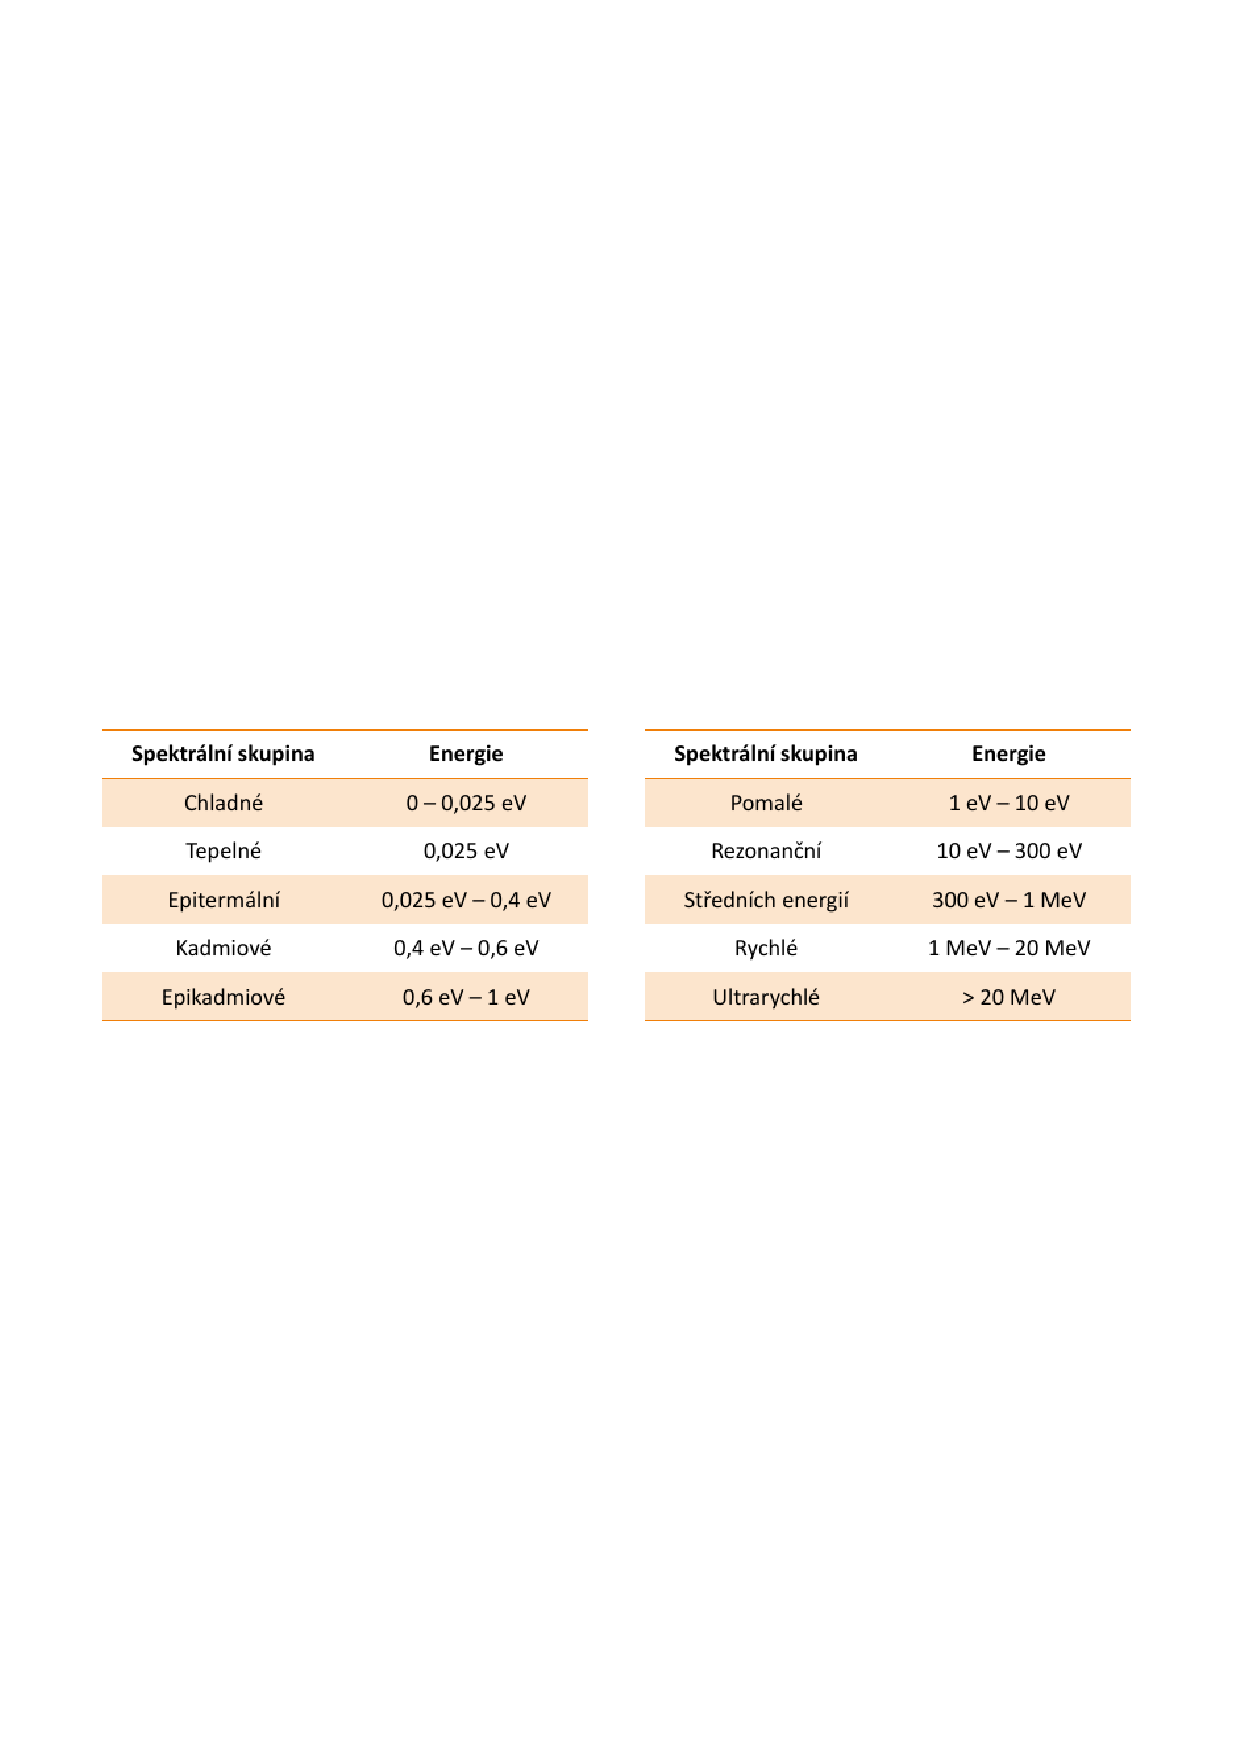
\includegraphics[width=0.8\linewidth, trim={1cm 12cm 1cm 12cm}, clip]{img/neutrony_energie.pdf}
    \caption{Rozdělení neutronů podle energie}
\end{figure}

\textbf{Měření indukované aktivity:}

\begin{itemize}
    \item Aktivita vzniklá v reakcích s neutrony $A(t)\,=\,n_{\text{R}} \cdot (1 - e^{-\lambda \cdot t})$.
    \item Může docházet k parazitním aktivačním reakcím $\rightarrow$ ovlivnění výsledků.
    \item Měření aktivity: koincidenční metodou $\beta-\gamma$ nebo počítání částíc v geometrii 4$\pi$.
    \item Rozsah většinou 10$^{10}$ až 10$^{22}$ cm$^{-2}$.
    \item Intermediální neutrony - rezonance $\rightarrow$ překryji detektor kadmiem $\rightarrow$ odfiltruji tepelné neutrony (kvůli ostrým maximům v $\sigma$).
    \item Rychlé neutrony $\rightarrow$ prahovými reakcemi.
\end{itemize}

\textbf{Počítání reakčních produktů:}

\begin{itemize}
    \item Většinou využívám (n,$\alpha$) nebo (n,p) případně (n,f) reakce.
    \item Fluence z počtu zaznamenaných částic (nutné určení účinnosti).
    \item Využívám u detektorů:
    \begin{itemize}
        \item scintilační,
        \item proporcionální počítače,
        \item štěpné komory,
        \item termoluminescenční,
        \item samonapájecí,
        \item fotografické emulze.
    \end{itemize}
\end{itemize}

\subsubsection{Detektory tepelných neutronů}

\begin{figure}[H]
    \centering
    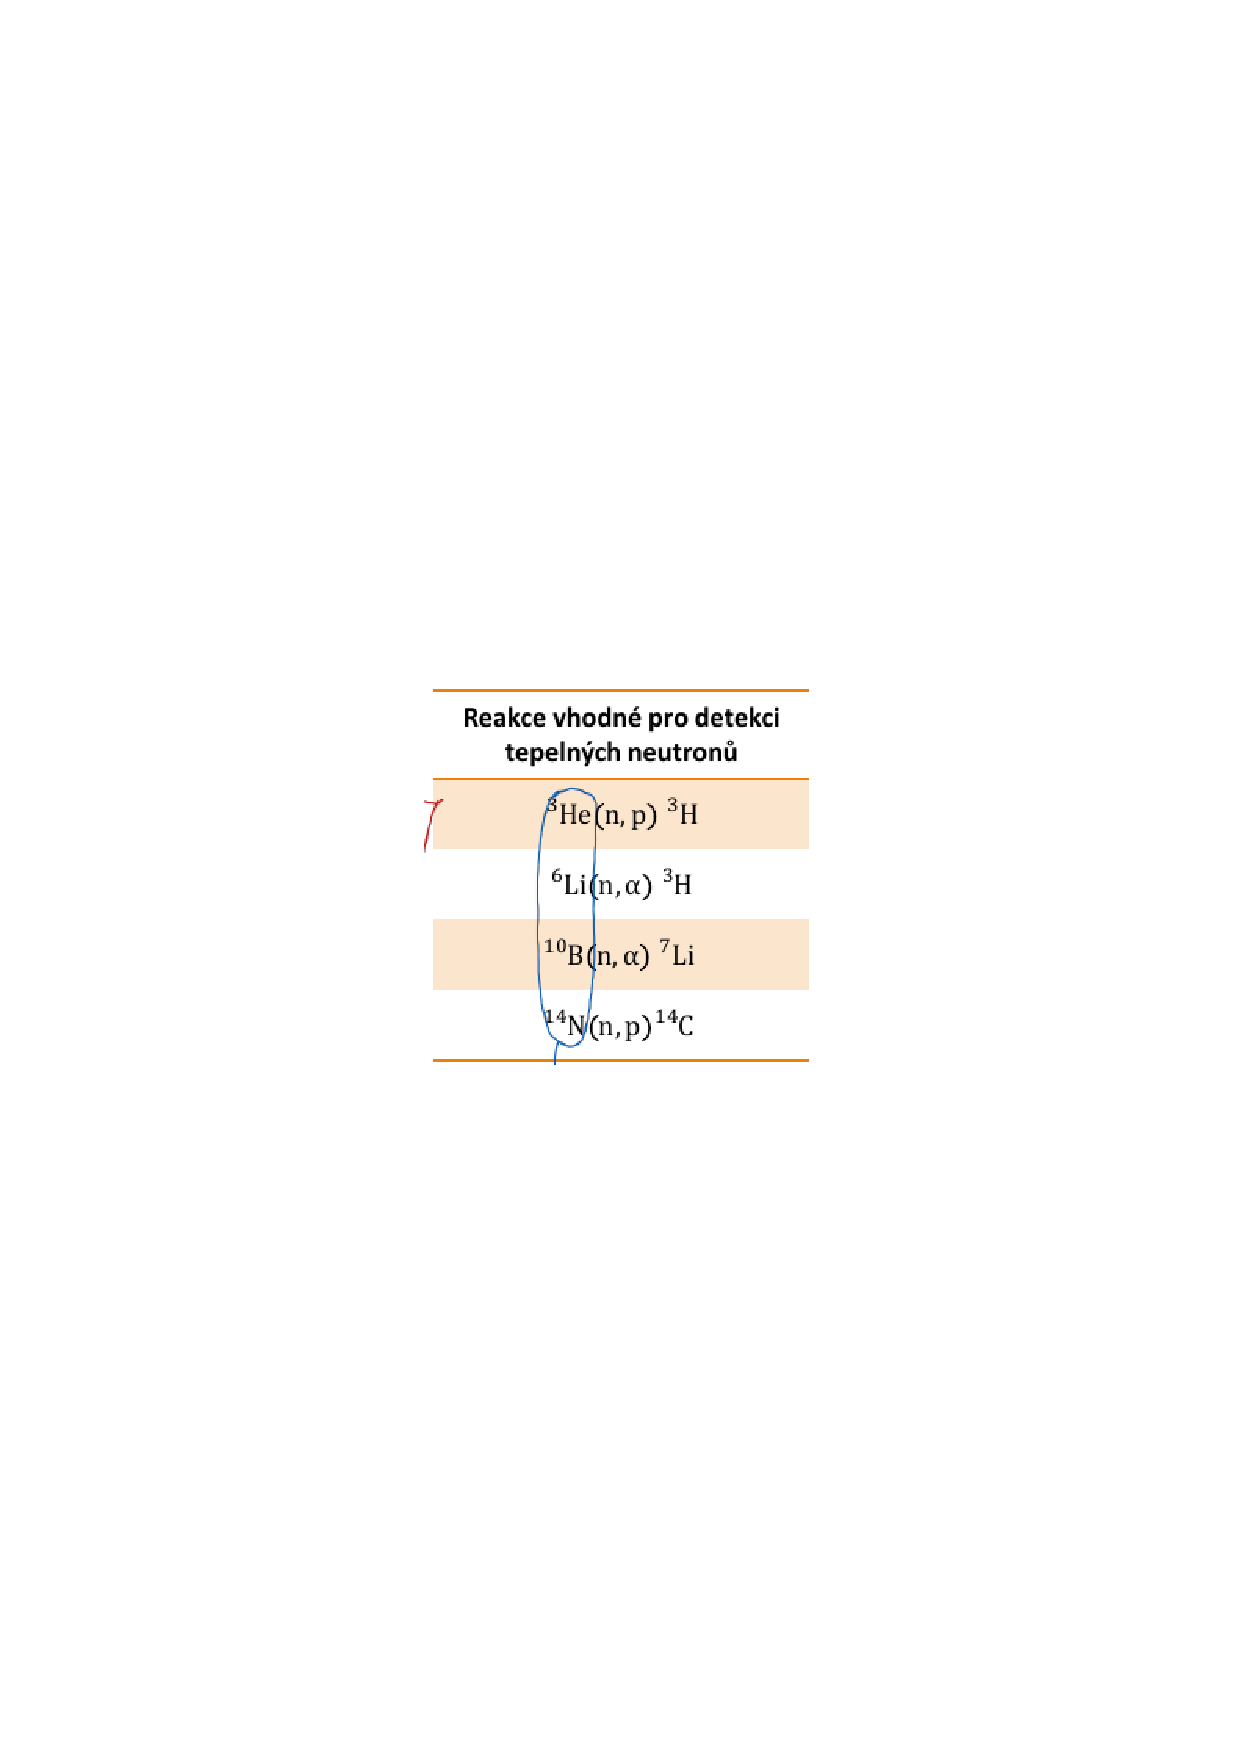
\includegraphics[width=0.4\linewidth, trim={5cm 12cm 5cm 12cm},clip]{img/reakce_tepelne_neutrony.pdf}
    \caption{Detekce tepelných neutronů -- reakce}
\end{figure}

\begin{itemize}
    \item Plynové:
    \begin{itemize}
        \item heliové a borové proporcionální komory - plynová náplň $^{3}$He a $^{10}$BF$_3$ nebo pokrytí stěny $^{10}$B,
        \item štěpné ionizační komory - stěny poryté obohaceným uranem (velká kinetická energie fragmentů),
    \end{itemize}
    \item scintilační -- konverzní materiál součástí scintilátoru (např. $^{6}$LiI(Eu)),
    \item polovodičové -- konverzní vrstva na povrchu detektoru,
    \item termoluminiscenční -- LiF obohacený o $^{6}$Li,
    \item detektory stop v pevné fázi,
    \item aktivační -- (n,$\gamma$),
    \item samonapájecí.
\end{itemize}

\subsubsection{Detektory rychlých neutronů}

\begin{itemize}
    \item Dlouhý počítač -- založeno an principu moderace.
    \item Závislost odezvy na energii nalétávající částice je "po dlouhou dobu stejná" od určité energie.
\end{itemize}

\subsection{Spektrometrie neutronů}

\begin{itemize}
    \item Většinou se používají Bonnerovy sféry.
    \item Detektor tepelných neutronů se umístí do středu PE koule s různým průměrem -- ty slouží jako moderátor.
    \item Postupně se naberou spektra.
    \item Následně $\rightarrow$ unfolding = proces, kdy je uhodnuté spektrum neutornů" jako vstup a je následně stanoveno "skutečné".
    \item Je to vleklá magie, náročné na měření.
    \item Na reaktoru používám pouze jednu bonnerku jako měřidlo dávkového příkonu.
\end{itemize}

Máme státní etalon \textbf{fluence neutronů} a \textbf{hustoty toku neutronů}.

\begin{itemize}
    \item Etalon fluence:
    \begin{itemize}
        \item zdroje neutronů: $^{252}$Cf, 1E8 s$^{-1}$ a AmBe 2E10 s$^{-1}$ a generátor 14 MeV 1E9 až 1E10 s$^{-1}$,
        \item kalibrační lavice, Bonnerův spektrometr,
        \item měřidlo prostorového dávkového ekvivalentu neutronů (to samé na VR-1 -- ta těžká bílá koule).
    \end{itemize}

    \item Etalon hustoty toku tepelných neutronů:
    \begin{itemize}
        \item grafitová prizma -- RN zdroje vkládám do moderujícího prostředí (viz neutronová laborka),
        \item vytvářím pole tepelných neutronů pro potřeby kalibrace a ověřování měřidel.
    \end{itemize}
\end{itemize}

\textbf{DOPSAT ZPRACOVÁNÍ VÝSLEDKŮ A ZDROJE NEJISTOT (ASI V JINÉ PREZENTACI)}




\section[Jaderná bezpečnost \& ochrana do hloubky]{Základní principy jaderné bezpečnosti a ochrana do hloubky}

\subsection{Princip 3S}

3S = Safety, Security, Safe Guards

Pro zajištění mírového a bezpečného využívání jaderné energie a prevenci zneužití jaderných materiálů je nezbytné vytvořit legislativní a regulační rámec. V této souvislosi se v oblasti jaderného průmyslu používají a aplikují tři sféry (pojmy), jež vyjadřují různé formy bezpečnosti:

\begin{itemize}
    \item \textbf{Bezpečnost/Safety} = Dodržovat provozní podmínky, předcházet nehodám a zmírňovat následky nehod. Vše s ohledem na ochranu pracovníků, veřejnosti a životního prostředí.

    V praxi to znamená, že zajistit bezpečný provoz znamená prokázat, že jaderné zařízení neohrožuje svým fungováním bezprostřední okolí ani zaměstnance a uživatele reaktoru.

    \underline{Příklad u nás na reaktoru VR1:} Bezpečnost jaderného zařízení je prokazována v oblasti jaderné bezpečnosti, radiační ochrany a havarijní připravenosti. Na pracovišti je vymezeno kontrolované pásmo, ve kterém je zabezpečeno nepřetržité monitorování prostředí i osob. Vstup do kontrolovaného pásma je povolen pouze poučeným osobám splňujícím podmínky vstupu. Prostor haly je monitorován systémem RMS (Radiační monitorovací systém), který je doplněn termoluminiscenčními detektory a potřebným množstvím přenosných přístrojů. Obsluha reaktoru je monitorována pomocí filmového a elektronického dozimetru, ostatní osoby vstupující do kontrolovaného pásma jsou vybaveny elektronickými dozimetry. Roční hodnota efektivní dávky od gama záření je pro pracovníky zpravidla menší než 0,5 mSv (povolená roční efektivní dávka pro radiační pracovníky je stanovena na 20 mSv za rok), u návštěvníků a studentů se pohybuje pod prahem citlivosti měřicích přístrojů

    \begin{itemize}
        \item \textbf{Jaderná bezpečnost} = Stav a schopnost jaderného zařízení a fyzických osob obsluhujícíh jaderné zařízení, aby byla zajištěna kontrola štěpné řetězové reakce, odvod tepla z AZ, zabránění úniku RA látek či IZ do ŽP a omezit následky nehod.

        Schopnost zařízení vychází z projektu a konstrukce zařízení, lze zvyšovat pravidelnou inovací a modernizací zařízení. Stav zařízení vystihuje aktuální stav zařízení. Zařízení je v dobrém stavu udržováno díky náležité údržbě a provozním kontrolám (např. kontrola reaktorových nádob a vnitřních částí, stav a provozuschopnost absorpčních tyčí nebo testy systému ochran řízení). Schopnost obsluhy hodnocena již při výběru vhodných pracovníků, kdy jsou hodnoceny odborné znalosti, ale také osobnostní charakteristiky. Schopnost obsluhy vychází z kvalitní odborné přípravy a je ověřována zkušební komisí SÚJB. Schopnost obsluhy je zvyšována (a ověřována) v rámci další odborné přípravy a periodického školení. Stav obsluhy dána aktuálním fyzickým stavem a psychickým rozpoložením. Díky pravidelnému ověřování osobnostní a zdravotní způsobilosti jsou vytvářeny podmínky, aby stav obsluhy odpovídal vysokým nárokům.

        \item \textbf{Radiační ochrana} = Ochrana pracovníků, veřejnosti a životního prostředí před rizikem ionizujícího záření pomocí technických a organizačních opatření.
        
        \item \textbf{Připravenost k odezvě na RMU} = Spojeno s rozpoznáním a reakcí na mimořádnou událost, která může při provozu vniknout.
        
        RMU = událost, která vede nebo může vést k překročení limitů ozáření a která vyžaduje opatření, jež by zabránila jejich překročení nebo zhoršování situace z pohledu zajištění radiační ochrany.

        \item \textbf{Radiační mimořádná událost prvního stupně} = RMU zvládnutelná silami a prostředky obsluhy nebo pracovníků vykonávajících práci v aktuální směně osoby, při jejíž činnosti radiační mimořádná událost vznikla.
        
        \item \textbf{Radiační nehoda} = RMU nezvládnutelná silami a prostředky obsluhy nebo pracovníků vykonávajících práci v aktuální směně osoby, při jejíž činnosti radiační mimořádná událost vznikla, nebo vzniklá v důsledku nálezu, zneužití nebo ztráty radionuklidového zdroje, která nevyžaduje zavedení neodkladných ochranných opatření pro obyvatelstvo.
        
        \item \textbf{Radiační havárie} = RMU nezvládnutelná silami a prostředky obsluhy nebo pracovníků vykonávajících práci v aktuální směně osoby, při jejíž činnosti radiační mimořádná událost vznikla, nebo vzniklá v důsledku nálezu, zneužití nebo ztráty radionuklidového zdroje, která vyžaduje zavedení neodkladných ochranných opatření pro obyvatelstvo.
        
    \end{itemize}

    \item \textbf{Zabezpeční/Security} = Prevence, detekce a včasná odezva na krádež, sabotáž, neautorizované vstupy, nelegální převoz a další akce zahrnující jaderné a radioaktivní materiály.
    
    Neboli: zabezpečení pracoviště je takové aby zabránilo k záměrnému zneužití či poškození zařízení a nebo k neoprávněným manipulacím s jaderným materiálem.

    \underline{Příklad u nás na reaktoru VR1:} Zabezpečení pracoviště vychází ze základních funkcí fyzické ochrany, jako je včasná detekce útočníka, jeho zpomalení a adekvátní zásah. Fyzická ochrana reaktoru a jaderných materiálů, které se na něm používají, splňuje požadavky vyhlášky SÚJB o zabezpečení jaderných materiálů a jaderných zařízení, která vychází z doporučení Mezinárodní agentury pro atomovou energii.

    \begin{itemize}
        \item \textbf{Fyzická ochrana} = Systém technických a organizačních opatření zabraňující neoprávněným činnostem s jaderným zařízením nebo jaderným materiálem.
        \item \textbf{Kybernetická bezpečnost} = Zajištění bezpečnosti kybernetického prostoru -- HW, SW, počítačové sítě, ...\item \textbf{Ochrana informací} = Ochrana a nakládání s citlivými informacemi, jsou to informace ovlivňující bezpečnost (omezené, důvěrné, tajné), souvisí s kybernetickou bezpečností a fyzickou ochranou.
    \end{itemize}
    
    \item \textbf{Zárukový proces/Safeguards} = Včasnou detekcí zneužití jaderných materiálů nebo technologií zabránit šíření jaderných zbraní, poskytnutí záruky, že státy využívají jaderný materiál a jaderná zařízení pouze pro mírové účely.

    Znamená: Reaktor, resp. jaderné zařízení musí být provozováno dle pravidel stanovených smlouvou o nešíření jaderných zbraní. Zárukový proces zajišťuje permanentní evidenci a kontrolu všech jaderných materiálů na pracovišti reaktoru.

    \underline{Příklad u nás na reaktoru VR1:} Základním kamenem zárukového procesu na pracovišti reaktoru je systém evidence a kontroly všech držených štěpných jaderných materiálů. Každá položka jaderného materiálu je sledována, má přesně definované místo svého uložení a svůj inventární záznam. Přesuny a manipulace jaderných materiálů lze provést pouze se souhlasem vedoucího evidence jaderných materiálů a tyto změny musí být zavedeny do evidenčních záznamů.

    Mezinárodní dohody členských států IAEA:

    \begin{itemize}
        \item \textbf{Treaty on the Non-Proliferation of Nuclear Weapon} = Dohoda o nešíření jaderných zbraní
        \item Dohoda o zárukách
        \item Výměna informací = Hlášení informací spojených se zárukovým procesem národním koordinátorům a IAEA.
    \end{itemize}

    \textbf{Forenzika} = Nástroje a metody pro vyšetřování zneužití jaderných materiálů, neschválené aktivity.

\end{itemize}

Může být těžké rozlišit bezpečnost a zabezpečení. \textbf{Zabezpečení} je spojeno se zlým úmyslem, cílenou akcí lidí, která může ohrozit další lidi, hrozba směřuje z okolí směrem do zařízení. \textbf{Bezpečnost} zahrnuje širší otázky ohrožení lidí (nebo životního prostředí) radiací, bez ohledu na primární příčinu, hrozba směřuje od zřízení směrem do okolí.

\subsection{Principy bezpečného využívání jaderné energie}

V rámci bezpečnosti jaderného zařízení, jehož součástí je jaderný reaktor je provozovatel (držitel lincence) nucen, aby bylo za každé situace zajištěno plnění základních bezpečnostních funkcí, přičemž v analýzách prokazování uvažuje jednoduchou poruchu a hermetičnost kontejmentu.

\subsubsection{Bezpečnostní funkce}

Splnění všech bezpečnostních funkcí je nezbytné pro zajištění jaderné bezpečnosti.

\begin{itemize}
    \item \textbf{Kritická bezpečnostní funkce} = ochrana celistvosti jedné nebo více fyzických bariér proti úniku RA látek.
    \item Musí být zachovány i při selhání nebo nesprávné činnosti jednotlivých zařízení a chybě obsluhy $\rightarrow$ musí být zahrnuto v projektu.
    \item Splnění základních bezpečnostních funkcí musí být zajištěno ve všech provozních stavech a ve všech etapách
    životního cyklu JZ.
\end{itemize}

Základní bezpečnostní funkce podle §45 odst. 2 AtZ, a §2 písm. b) vyhl. 329/2017 Sb.:

\begin{itemize}
        \item umožňovat v případě potřeby okamžitě a bezpečně odstavit jaderný reaktor a udržovat jej v podkritickém stavu
        \item zabránit nekontrolovanému rozvoji štěpné řetězové reakce
        \item fyzikálně znemožnit vznik kritického a nadkritického stavu mimo vnitřní prostor jaderného reaktoru
        \item zajišťovat odvod tepla vytvářeného jaderným palivem a technologickými systémy
        \item zajistit stínění a zabránit úniku radioaktivní látky a šíření ionizujícího záření do životního prostředí
    \end{itemize}

Základní bezpečnostní principy:

\begin{itemize}    
	\item \textbf{Administrativní opatření} = opatření pro řízení a ověřování bezpečnosti
 
	\item \textbf{Technická opatření} = technické principy uplatněné v celém životním cyklu zařízení
        \begin{itemize}
            \item \textbf{Diverzita} = různorodost, různé principy, technologie, výrobci $\rightarrow$ snaha o vyloučení poruchy ze společné příčiny
             \item \textbf{Redundance} = zálohování, vícenásobné použití $\rightarrow$ omezení jednoduché poruchy, eliminace stochastických poruch
            \item \textbf{Nezávislost} = využití rozdílných metod, zdrojů
            \item \textbf{Separace} = fyzické oddělení systémů $\rightarrow$ ochrana proti externím vlivům (společná příčina)
        \end{itemize}
 
    \item \textbf{Kultura bezpečnosti} = Soubor charakteristik a postojů organizace i jednotlivců zajišťující, že otázkám ochrany a bezpečnosti je věnována priorita odpovídající jejich významu. Individuální i kolektivní závazek k bezpečnosti ze strany personálu na všech úrovních (včetně vedení a středního managementu). Odpovědnost organizace i jednotlivců za dodržování pravidel bezpečnosti. Podpora vzdělávání a budování prostředí otevřeného dotazům spojeným s plněním bezpečnosti. Chování managementu funguje jako vzor v pozitivním i negativním smyslu.

    Principy kultury bezpečnosti:

    \begin{itemize}
        \item Individuální i kolektivní závazek k bezpečnosti ze strany personálu na všech úrovních (včetně vedení a středního managementu).
        \item Osobní odpovědnost za bezpečnost.
        \item Vedoucí pracovníci demonstrují svoje postoje k bezpečnosti.
        \item Respekt vůči jaderné technologii.
        \item Při rozhodování platí "bezpečnost na prvním místě".
        \item Trvalé ověřování úrovně bezpečnosti..
        \item Poučení se z chyb
    \end{itemize}
\end{itemize}

\subsubsection{Přístup třístupňové ochrany}

\begin{itemize}
    \item \textbf{Prevence} = Základ všeho. Předchází vzniku problémů a snahou je vyhnout se provozním stavům, které mohou vést k poškození paliva/AZ a úniku RA látek. Jedná se tak např. o: Využívání inherentních prvků (např. záporné koeficienty reaktivity), ochrané a bezpečnostní limity, pravidelné bezpečnostní hodnocení, výcvik a zajištění jakosti (dobré materiály, pořádný projekt, připravenost na nejrůznější scénáře).
    \item \textbf{Ochrana} = zabránit nebo potlačit nepříznivé jevy, málo pravděpodobné události a přechodové procesy, které mohou vést k poškození paliva a malým únikům RA látek. Zařízení musí mít k dispozici systémy pro zvládnutí všech myslitelných událostí (postulované události).
    \item \textbf{Zmírnění následků} = zahrnuje bezpečnostní systémy a systémy pro zvládání těžkých nehod, které mají zastavit nebo maximálně omezit dopady na obyvatelstvo a ŽP.
\end{itemize}

\subsubsection{Definice poruch}

\begin{itemize}
    \item \textbf{Jednoduchá porucha} = událost vedoucí ke ztrátě schopnosti prvku zařízení vykonávat svou funkci, ale ostatní prvky pracují správně.
    \item \textbf{Porucha ze společné příčiny} = porucha nebo selhání dvou a více prvků zařízení ze stejné příčiny.
    \item \textbf{Deterministická porucha} = lze identifikovat a odstranit, chyby obsluhy, v projektu, v konstrukci, ve výpočtech.
    \item \textbf{Stochastická porucha} = nahodilá, nejsou předem známy důvody, např. nedosednutí odlehčovacího ventilu.
\end{itemize}

\subsubsection{Rozdělení systémů}

\begin{itemize}
    \item \textbf{Aktivní systémy} = činnost aktivních prvků, vyžadují zdroj el. energie, např. spuštění čerpadla.
    \item  \textbf{Pasivní systémy} = samovolný účinek, neobsahují aktiv. prvky, netřeba pohon či zdroj, např.~hydroakumulátory.
    \item  \textbf{Inherentní opatření} = využití fyzikálních zákonů a principů, např. snížení moderace při zvýšení teploty.
\end{itemize}

\subsection{Ochrana do hloubky = DID}

Ochrana do hloubky představuje soubor nezávislých a postupně odstupňovaných úrovní projektových opatření zálohující zajištění základních bezpečnostních funkcí. Je založena na deterministčiných předpokladech a postupech, ale uvažuje odstupňovaný přístup vycházející z pravděpodobnosti jednotlivých událostí. Narušení funkce projektových opatření v rámci jedné úrovně musí být rozpoznáno a napraveno nebo kompenzováno dalšími nezávislými projektovými opatřeními, implementovanými v následných úrovních.

Ochrana do hloubky je založena na sestavení fyzických bariér mezi zdrojem IZ a životním prostředí. Samotné fyzické bariéry nejsou dostatečné, mohou selhat $\rightarrow$ je potřeba prostředky na ochranu jednotlivých bariér (bezpečnostní systémy, technické a organizační opatření).

Při správné implementaci žádná jednotlivá porucha, lidská nebo organizační chyba nevede ke škodlivým účinkům, přičemž základní podmínkou je vzájemná nezávislost jednotlivých úrovní ochrany do hloubky.

\subsubsection{Zajištění DID}

\begin{itemize}
    \item Efektivní systém řízení se silným závazkem vůči bezpečnosti a dodržování pravidel kultury bezpečnosti.
    \item Vhodná lokalita pro umístění zařízení, dobrý návrh zařízení doplněný bezpečnostními systémy s využitím diverzity a redundance -- technologie a materiály vysoké kvality a spolehlivosti, řídicí, limitační a ochranný systém, kombinace inherentní bezpečnosti a bezpečnostních systémů.
    \item Bezpečnostní systémy jsou poslední část prostředků, které zajišťují udržení filozofie ochrany do hloubky.
\end{itemize}

\subsubsection{Strategie DID}

Více úrovňovou strategii ochrany do hloubky lze shrnout následovně:

\begin{itemize}
    \item Předejít a zabránit selhání, poruchám a nehodám.
    \item Pokud dojde k selhání, zabránit rozvoji nehody a zmírňovat následky.
    \item Kompenzace potenciálních lidských chyb a selhání zařízení.
    \item Udržet efektivitu bariér a ochránit veřejnost a ŽP.
    \item Nezávislost jednotlivých úrovní.
\end{itemize}

\subsubsection{Úrovně DID}

Konkrétní bezpečnostní úrovně ochrany do hloubky jsou následující:

\begin{itemize}
	\item[1)] Úroveň = Zabránění vzniku abnormálních stavů a selhání systémů důležitých z hlediska bezpečnosti $\rightarrow$ prevence.

        \begin{itemize}
            \item Design zařízení, konstrukce, údržba, způsob provozu -- konzervativní přístup.
            \item Definice podmínek, které vedou k nechtěným únikům.
            \item Zvážení vnitřních a vnějších rizik.
            \item 1) úroveň ochrany do hloubky je zajišťována normálními provozními systémy.
        \end{itemize}

	\item[2)] Úroveň = Kontrola abnormálních stavů a detekce poruch.

        \begin{itemize}
            \item Aplikace postupů pro zvládání odchylek od normálního provozu, postupy pro rychlý návrat do normálu. Využívá se i inherentní bezpečnosti.
            \item Zajišťuje včasnou detekci selhání, kontrolu nad vznikem abnormálního provozu a co nejrychlejší navrácení provozu do běžného stavu.
            \item Periodické kontroly zařízení a údržba, nedestruktivní testování.
            \item Ochranné systémy: snížení výkonu, automatické odstavení, předpisy pro abnormální provoz, systém limitování maximálního výkonu reaktoru, systém kontroly teploty, pojišťovací ventily zamezující velkému převýšení tlaku v primárním a  ekundárním okruhu a další řídící a limitační systémy.
            \item 2) úroveň ochrany do hloubky je zajišťována normálními provozními systémy
        \end{itemize}

	\item[3)] Úroveň =  Kontrola projektových nehod (DBA), zabránění poškození AZ, lokalizace RA látek.
 
        \begin{itemize}
            \item Bezpčnostní systémy pro zvládání projektových havárií, tyto systémy mají pedevším zabezpečit dostatečné chlazení aktivní zóny a tím předejít jejímu taven.
            \item Aplikace základních bezpečnostních principů (diverzita, redundance,separace, nezávislost).
            \item Prevence chyb se společnou příčinou, a jednoduché chyby.
            \item Bezpečnostní systémy mají za cíl bránit vzniku DBA, zvládat DBA a bránit především jejich rozvoj do BDBA/DEC A, tj. potlačují rozvoj poruch zařízení a chyb obsluhy.
            \item Řízení havárie je dáno projektem a probíhá podle havarijních provozních předpisů.
            \item Bezpečnostní systémy: systémy havarijního chlazení AZ, systém nouzového napájení PG, systém snižování tlaku v IO (přepouštěcí stanice), systém lokalizace následků havárie (kontejnment, barbotážní věž).
        \end{itemize}

    \item[4)] Úroveň = Kontrola havarijních stavů (BDBA/DEC B, SA), prevence rozvoji havárie do radiační havárie, omezování následků vážných havárií a udržení celistvosti KTMT.
        
    Cílem 4) úrovně je, za předpokladu, že první tři úrovně ochrany do hloubky nezabrání poškození aktivní zóny, minimalizovat následky nadprojektové havárie a zabránit úniku radioaktivních látek do životního prostředí. 

        \begin{itemize}
            \item Cíl je zabránit velkému úniku RA látek z AZ.
            \item Ochrana kontejnmentu (chlazení, ventilace).
            \item Využití nestandardních prostředků (např. mobilní DG, požární voda pro sekundární chlazení) -- významná role operátorů.
            \item Bezpečnostní systémy pro zvládání těžkých havárií: lapač roztavené AZ, systém kontroly vodíku -- rekombinátory vodíku, systém pasivního odvodu tepla z KTMT, dodatečné filtrační systémy.           
        \end{itemize}

    \item[5)] Úroveň =  Omezování radiačních následků pro pracovníky a obyvatelstvo při významném úniku RA látek (radiační havárie)

        \begin{itemize}
            \item Tvoří havarijní plány a prostředky pro jejich realizaci, sloužící pro co největší zmírnění následků havárie (evakuace, likvidace havárie atd.).
            \item Shromažďování a hodnocení informací o úrovni očekávaných expozic.
            \item Krátkodobé a dlouhodobé ochranné akce, příprava adekvátní reakce na situaci (zapojení zodpovědných úřadů).
            \item Ukrytí, evakuace, jódová profylaxe, kontrola zemědělství a rybolovu.
            \item Řízení připravenosti k odezvě, havarijní plánování, vnitřní a vnější havarijní plán.
        \end{itemize}

\end{itemize}

\begin{figure}[h!]
    \centering
    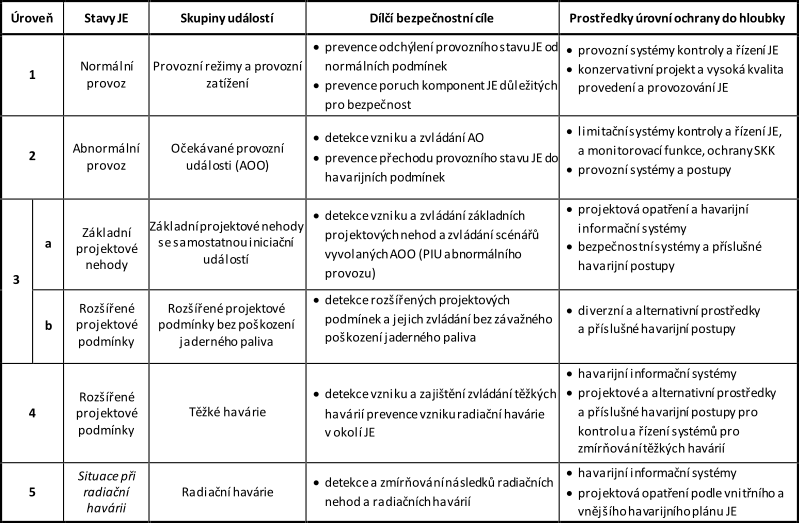
\includegraphics[width=\textwidth]{img/Úrovně ochrany do hloubky.png}
    \caption{Úrovně ochrany do hloubky.}
\end{figure}

\subsubsection{Fyzické bariéry DID}

Počet jednotlivých bariér závisí na zdrojovém členu (ETE jich má 5), účinnosti bariér, pravděpodobnosti výskytu a závažnosti nepříznivých interních i externích událostí.

Projekt musí zabránit ohrožení integrity fyzických bariér, a to zejména poslední a tím zabránit úniku RA látek do ŽP. Cílem je však zamezení selhání jedné nebo více bariér při ohrožení.

Vyloučit závislost, tj. zabránit selhání jedné bariéry v důsledku selhání jiné bariéry (stejné jako pro jednotlivé úrovně DID).

Není dovolen provoz při selhání jedné z bariér (jedná se o výzmnou událost a je nutné prošetřit).

\begin{enumerate}
	\item Palivová tableta -- chemická a fyzikální struktura paliva.
	\item Pokrytí palivových proutků -- hermetická hranice.
	\item Tlaková hranice primárního okruhu.
	\item Kontejnment (nebo jiný systém lokalizace RA látek pokud nemám kontejment $\rightarrow$ barbotážní věž).
\end{enumerate}

\begin{figure}[h!]
    \centering
    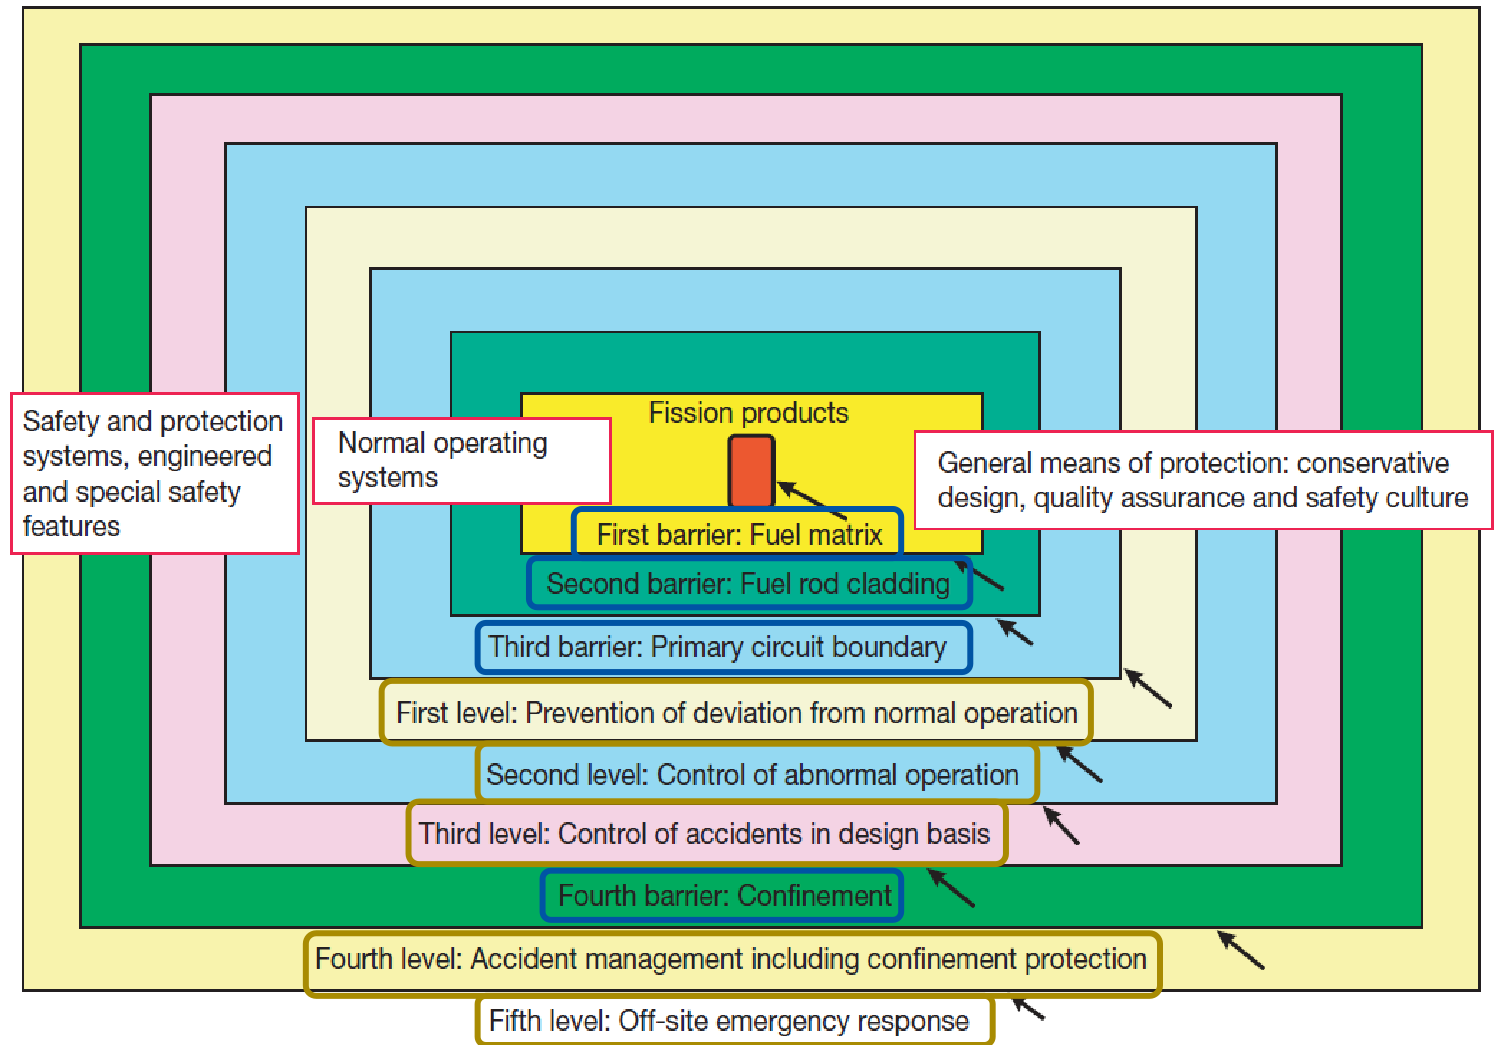
\includegraphics[width=\textwidth]{img/DiD-bariery.png}
    \caption{Bariéry a úrovně ochrany do hloubky.}
\end{figure}
\section[Klasifikace událostí na jaderných zařízeních]{Klasifikace událostí na jaderných zařízeních a rozbor vybraných událostí}


\section[Legislativa jaderné bezpečnosti]{Postavení provozovatele, státního dozoru a IAEA v jaderné bezpečnosti, legislativní rámec jaderné bezpečnosti}

\end{document}
